% !TEX TS-program = lualatex

\documentclass[14pt,russian,a4paper]{extreport}
 
\input{../preamble_bmstu_lua.tex}

\usepackage{geometry}
\geometry{left=3cm}
\geometry{right=2cm}
\geometry{top=2cm}
\geometry{bottom=2.2cm}

\addbibresource{biblio.bib}

\usepackage{tikz}
\newcommand*\circled[1]{\tikz[baseline=(char.base)]{
             \node[shape=circle,draw,inner sep=2pt, minimum size=8mm] (char) {#1};}}

\cfoot{}
\rfoot{\thepage}
\fancypagestyle{plain}{ 
    \fancyhf{}
    \cfoot{}
    \rfoot{\thepage}}


\linespread{1.4} % полуторный интервал
\frenchspacing

\setcounter{tocdepth}{1}

\titleformat{\chapter}
    {\filcenter\normalsize\bfseries}{\thechapter}{0.7em}
    {\trackedcaps}

\faculty{М-КФ «Машиностроительный»}
\department{М1-КФ «Машиностроительные технологии»}
\reportname{Курсовой проект}
\discipline{Основы конструирования приспособлений}
\thetopic{Проектирование станочных приспособлений}
\writtenby{студент группы ТМД.Б-71 Куркин М. В.}
\checkedby{Попков В. М.}
\thefooter{Калуга, 2018 г.}

\begin{document}

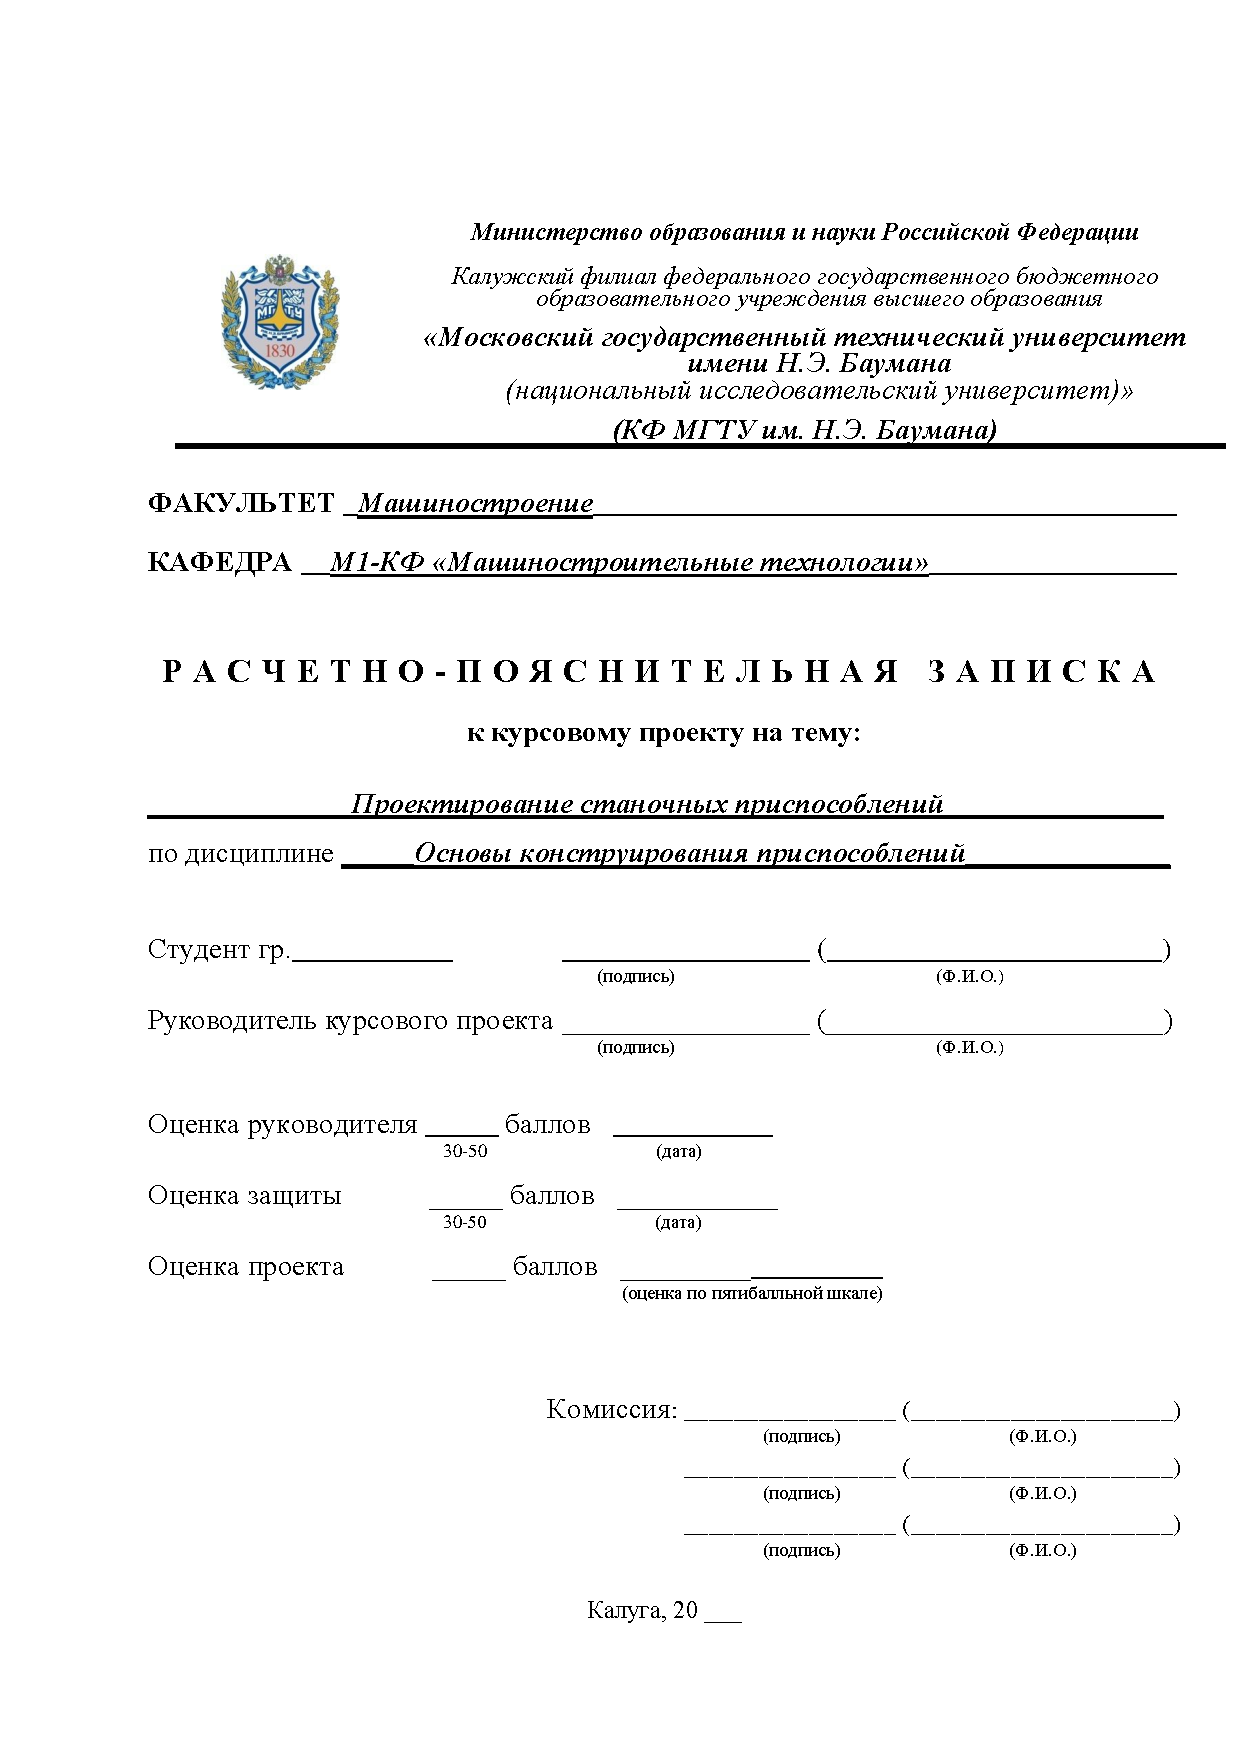
\includepdf[pages=1,offset=-5mm 8mm,angle=0,scale=1.00]{./graphics/7_kp_title.pdf}
\includepdf[pages=2,offset=-5mm 0mm,angle=0,scale=1.00]{./graphics/7_kp_title.pdf}

\setcounter{page}{3}

\tableofcontents

\chapter{Анализ исходных данных}

\section{Служебное назначение детали}

Обрабатываемая деталь --- корпус барабана. Детали типа «корпус» предназначены для крепления к ним других деталей и сборочных единиц изделия. Корпусные детали обеспечивают точность и постоянство относительного расположения прикрепляемых к ней деталей, поэтому должны обладать достаточной жёсткостью. Обрабатываемая деталь является вращающейся.\par

Наружная поверхность детали --- призма, основанием которой является правильный шестиугольник с диаметром вписанной окружности $\SI{620}{\milli\meter}$. С обеих торцов призмы деталь имеет ряд выступов, образующих цилиндрические и конические поверхности. На каждой грани шестигранника расположено по четыре штифтовых отверстия $\SI{20}[\diameter]{H7 \; \milli\meter}$ и по восемь резьбовых M12. \par

Ступица детали имеет отверстие $\SI{125}[\diameter]{H7 \; \milli\meter}$, предназначенное для ус\-тановки детали на вал. На внешней части ступицы расположен паз. Ступица соединена с наружной частью детали полотном. На нём расположены 6 рёбер, служащих для повышения жёсткости детали. В перемычках между спицами выполнены два такелажных отверстия $\SI{100}[\diameter]{\milli\meter}$.  \par

Кроме перечисленных, деталь имеет ряд резьбовых и штифтовых отверстий, необходимых для прикрепления к корпусу других деталей изделия. \par

Заготовка детали --- отливка из серого чугуна СЧ~21-40 (ГОСТ~1412-85). \par



\section{Анализ технических условий на изготовление~детали}

Наиболее точные цилиндрические поверхности детали --- отверстие в ступице $\SI{125}[\diameter]{H7 \; \milli\meter}$, 6 отверстий $\SI{45}[\diameter]{H7 \; \milli\meter}$, 2 отверстия $\SI{25}[\diameter]{H7 \; \milli\meter}$, 26 отверстий $\SI{20}[\diameter]{H7 \; \milli\meter}$ и 6 отверстий $\SI{12}[\diameter]{H7 \; \milli\meter}$. Необходимость их высокой точности обусловлена тем, они являются сопрягаемыми. Для менее точных поверхностей заданы их предельные отклонения: $\SI{600}[\diameter]{_{-0,2} \; \milli\meter}$ и $\SI{590}[\diameter]{_{-0,5} \; \milli\meter}$. Заданные предельные отклонения удовлетворяют требованиям, соответственно, 10 и 12 квалитетов. Размеры с неуказанными предельными отклонениями выполняются по 14 квалитету. \par

Точность взаимного расположения поверхностей детали задана допусками параллельности торцовых поверхностей детали относительно друг друга и перпендикулярности наружных граней корпуса относительно торца, которые составляют $\SI{0,03}{\milli\meter}$, и допуском радиального биения наружной цилиндрической поверхности $\SI{600}[\diameter]{_{-0,2} \; \milli\meter}$ относительно посадочного отверстия ступицы $\SI{125}[\diameter]{H7 \; \milli\meter}$, который составляет $\SI{0,1}{\milli\meter}$. \par

Точность формы задана допусками на плоскостность торца и наружных граней корпуса, который составляет $\SI{0,02}{\milli\meter}$. \par

Шероховатость задана значениями Ra~1,25 для посадочного отверстия ступицы $\SI{125}[\diameter]{H7 \; \milli\meter}$ и других сопрягаемых отверстий, Ra~2,5 для плоских поверхностей наружных граней и торцов корпуса и для внутренней цилиндрической поверхности $\SI{430}[\diameter]{\milli\meter}$, и Ra~10 для плоских поверхностей торцов ступицы, наружных цилиндрических поверхностей $\SI{590}[\diameter]{_{-0,5} \; \milli\meter}$ и отдельных резьбовых отверстий. Для остальных поверхностей задана шероховатость Rz~630, получаемая без применения механической обработки.


\section{Характеристика материала заготовки}

Материал заготовки --- серый чугун СЧ~21-40 (ГОСТ~1412--85). Это чугун с пластинчатым графитом для отливок с временным сопротивлением при растяжении не менее $\sigma_B = \SI{210}{\mega\pascal}$. \par

Серый чугун --- сравнительно дешёвый конструкционный материал. Имеет хорошие литейные и технологические свойства. Из серого чугуна изготавливают массивные литые детали, такие как станины, маховики, крупногабаритные корпуса. \par

Физические свойства чугуна СЧ~21-40: плотность $\rho = \SI{7100}{\kilo\gram\per\meter\cubed}$, линейная усадка $\varepsilon = \SI{1,2}{\percent}$, модуль упругости при растяжении $E = \SIrange[allow-number-unit-breaks]{850}{1100e-5}{\mega\pascal}$, удельная теплоёмкость при $t = \SIrange{20}{200}{\celsius}$ $c = \SI{480}{\joule\per\kilo\gram\per\kelvin}$, коэффициент линейного расширения при $t = \SIrange{20}{200}{\celsius}$ $\alpha = \SI[per-mode=reciprocal]{9,5e-6}{\per\celsius}$, теплопроводность при $\SI{20}{\celsius}$ $\lambda = \SI{54}{\watt\per\meter\per\kelvin}$. \par

Химический состав чугуна СЧ~21-40: массовая доля углерода $\SIrange{3,3}{3,5}{\percent}$, кремния --- $\SIrange{1,4}{2,4}{\percent}$, марганца --- $\SIrange{0,7}{1,0}{\percent}$, фосфора --- не более $\SI{0,2}{\percent}$, серы --- не более $\SI{1,5}{\percent}$. Допускается низкое легирование чугуна различными элементами (хромом, никелем, медью, фосфором и другими).


\section{Анализ технологичности конструкции детали}

Большинство конструктивных элементов детали унифицированы. 

Точность размеров и шероховатость поверхностей экономически и конструктивно обоснованы. 

Физико-химические и механические свойства материала, жёсткость детали, её форма и размеры соответствуют требованиям технологии изготовления, конструкция жёсткая.

Деталь имеет технологические базы, позволяющие обеспечить точность установки, обработки и контроля.

Обработка и контроль точных поверхностей детали не затруднены.

Деталь имеет большое количество глухих точных отверстий, что усложняет обработку.

Шпоночный паз расположен нетехнологично, его обработка затрудняется необходимостью располагать деталь под углом.

Большая масса и габаритные размеры заготовки усложняют транспортировку и установку детали на станке.

Конструкция детали в целом технологична, но имеет ряд элементов, обработка которых затруднена.


\chapter{Проектирование операций механической обработки детали}

\section{Проектирование сверлильной операции с ЧПУ}

\subsection{Выбор и характеристика оборудования}
Операция выполняется на горизонтальном сверлильно\-/фрезерно\-/расточном станке с ЧПУ и АСИ 2206ВМФ4. 

Это станок с крестовым поворотным столом, предназначенный для комплексной обработки плоских деталей средних размеров сложной формы. Станок предназначен для многооперационной обработки разнообразных деталей сложной конфигурации из стали, чугуна, цветных и лёгких сплавов. На станке можно производить получистовое и чистовое фрезерование плоскостей, пазов и криволинейных поверхностей различными типами фрез, а также растачивание, сверление, зенкерование, развёртывание отверстий и нарезание резьбы метчиками и резцами по заданной программе. Станок может быть использован в мелкосерийном и серийном производствах различных отраслей промышленности.

Управление станком --- от универсальной комплексной системы ЧПУ «Размер-2М-1300», позволяющей производить позиционную и контурную обработку, а также вручную с пульта управления. На станке программируются координатные перемещения стола и шпиндельной головки, скорости этих перемещений, частота вращения шпинделя, выбор и смена инструмента, смена обрабатываемой детали и циклы обработки.

На станке программируются координатные перемещения стола, шпиндельной головки, скорости этих перемещений, режимы обработки, выбор, смена и коррекция инструмента, циклы обработки.

Станок может быть оснащен устройством автоматической загрузки и выгрузки изделий, предназначенным для установки заготовки вне станка на сменные столы (паллеты) и последующей автоматической загрузки столов на станок, а также их выгрузки со станка после окончания обработки. Использование сменных столов устройства позволяет совместить загрузку заготовок или выгрузку обработанных изделий с работой станка, что существенно сокращает холостые простои, повышает эффективность его использования и производительность, при этом исключается последняя ручная операция --- установка и снятие деталей со станка.

Основные характеристики станка:
\begin{itemize}
  \item Класс точности станка В по ГОСТ 8-82
	\item Размеры рабочей поверхности стола $\SI{630 x 800}{\milli\meter}$
  \item Расстояние от торца шпинделя до центра стола $\SIrange{195}{825}{\milli\meter}$
	\item Наибольшее продольное перемещение стола (X) $\SI{800}{\milli\meter}$
	\item Наибольшее поперечное перемещение стола (Z) $\SI{630}{\milli\meter}$
	\item Наибольшее вертикальное перемещение шпиндельной головки (Y) $\SI{630}{\milli\meter}$
	\item Наибольшая нагрузка на стол $\SI{800}{\kilo\gram}$
	\item Ёмкость инструментального магазина $\SI{30}{\pcs}$
	\item Наибольший диаметр устанавливаемого инструмента $\SI{200}{\milli\meter}$
	\item Наибольшая длина инструмента, устанавливаемого в шпинделе станка $\SI{400}{\milli\meter}$
	\item Частота вращения шпинделя $\SIrange{10}{3500}{\rev\per\minute}$
	\item Электродвигатель привода шпинделя $\SI{15}{\kilo\watt}$
	\item Масса станка $\SI{12}{\tonne}$
\end{itemize}

\newpage
На рис.~\ref{fig:2206} приведены габариты рабочего пространства сверлильно\-/фрезерно\-/расточного станка 2206ВМФ4 (\subref{subfig:2206a}) и его посадочные и присоединительные размеры (\subref{subfig:2206b}, \subref{subfig:2206c}, \subref{subfig:2206d}).

\begin{figure}[H]
	\centering
  \begin{subfigure}[b]{.50\textwidth}
    \centering
    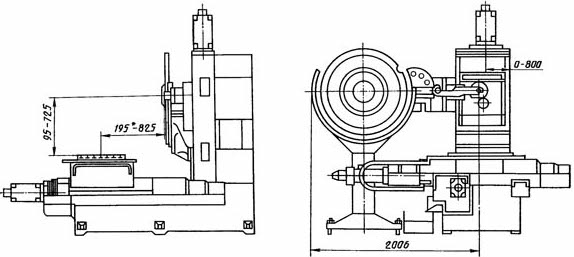
\includegraphics[width=.90\linewidth]{spr_2206vmf4_1.jpg}
    \caption{габаритные размеры рабочего поля}
    \label{subfig:2206a}
  \end{subfigure}%
  \begin{subfigure}[b]{.50\textwidth}
    \centering
    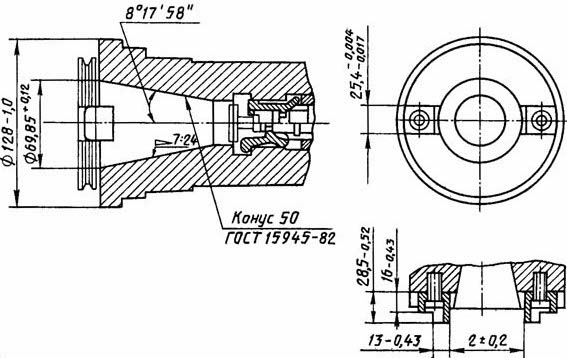
\includegraphics[width=.90\linewidth]{spr_2206vmf4_2.jpg}
    \caption{посадочные и присоединительные базы}
    \label{subfig:2206b}
  \end{subfigure} \\
  \begin{subfigure}[b]{.50\textwidth}
    \centering
    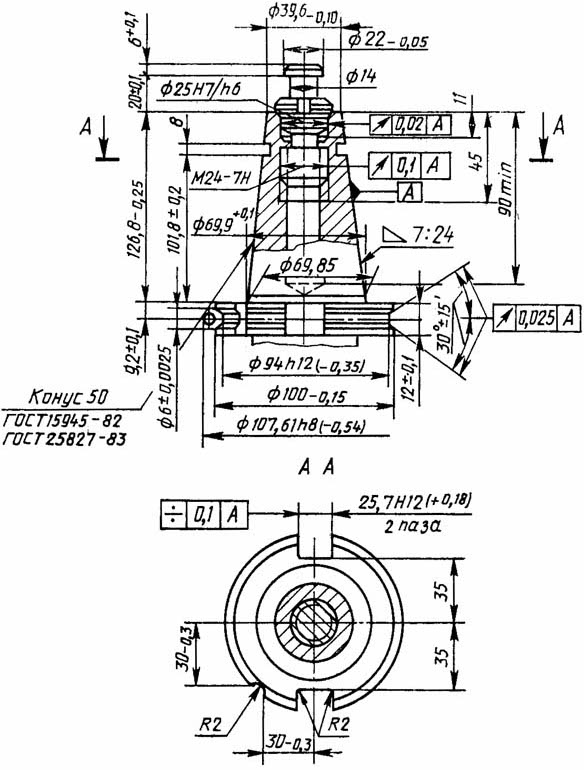
\includegraphics[width=.90\linewidth]{spr_2206vmf4_3.jpg}
    \caption{конец инструмента}
    \label{subfig:2206c}
  \end{subfigure}%
  \begin{subfigure}[b]{.50\textwidth}
    \centering
    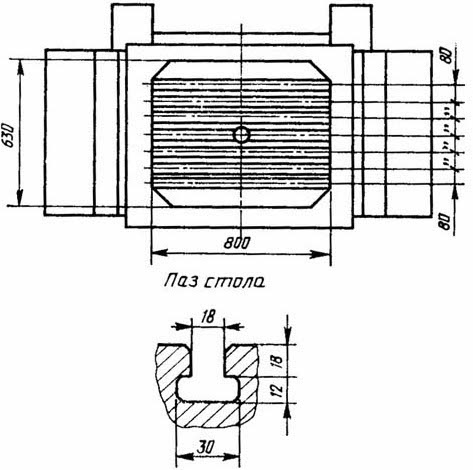
\includegraphics[width=.90\linewidth]{spr_2206vmf4_4.jpg}
    \caption{рабочий стол}
    \label{subfig:2206d}
  \end{subfigure}%
  \caption{Посадочные и присоединительные размеры станка 2206ВМФ4}
  \label{fig:2206}
\end{figure}

\newpage
\subsection{Выбор и обоснование схемы базирования}

Базирование осуществляется по схеме, представленной на рис.~\ref{fig:b040}

\begin{figure}[H]
	\centering
	   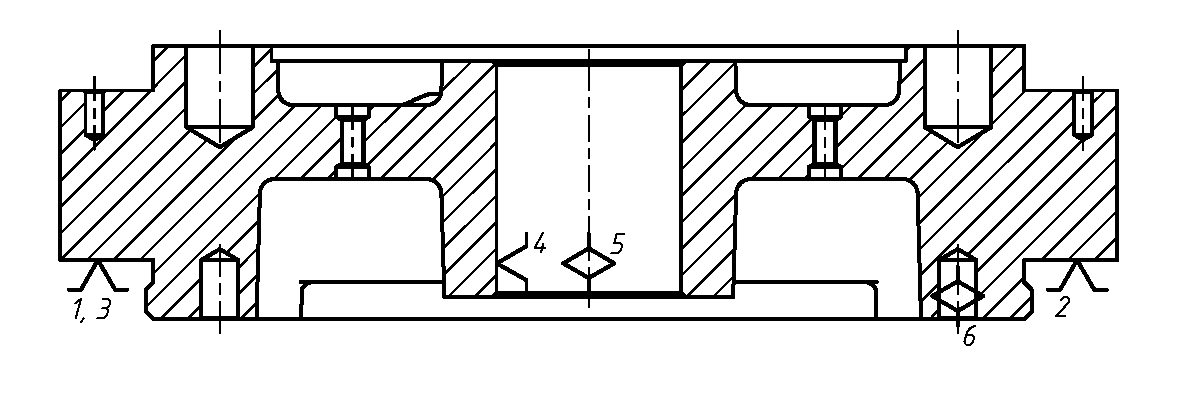
\includegraphics[width=0.7\textwidth]{bases_040.pdf}
	   \caption{Схема базирования на операции 040}
	   \label{fig:b040}
	   1, 2, 3 --- установочная база, \\
	   4, 5 --- направляющая база, \\
	   6 --- опорная база
\end{figure}

\subsection{Выбор и обоснование последовательности и содержания переходов}

На операции 040 осуществляется обработка отверстий, расположенных на гранях наружной поверхности детали. Деталь установлена в специальном приспособлении, поворот относительно своей оси она осуществляет за счёт делительного движения, совершаемого поворотным столом станка. На каждой позиции последовательно обрабатываются все отверстия, расположенные на грани, обращённой к шпинделю. Обработка 4 отверстий $\SI{20}[\diameter]{H7 \; \milli\meter}$ осуществляется за три перехода последовательным сверлением, зенкерованием и развёртыванием. Обработка 8 резьбовых отверстий M12-7H производится сверлением и нарезанием резьбы метчиком. Последним переходом снимаются фаски на всех отверстиях. После этого стол станка поворачивается и обрабатывается следующая грань детали. Последовательность обработки отверстий на каждой грани приведена в табл.~\ref{tab:040}.

\begin{table}[H]
  \setlength{\tabulinesep}{1.2ex}
  \begin{longtabu} to \textwidth { | X[7,l,p] | }
    \caption{Содержание основных переходов операции 040} \label{tab:040} \\
  
      \hline 
      \multicolumn{1}{|c|}{\linespread{1.1} \bfseries{\small Содержание переходов}} \\ \hline 
    \endfirsthead
  
      \multicolumn{1}{l}{{\itshape Продолжение таблицы \thetable{}}} \\ \hline 
      \multicolumn{1}{|c|}{\linespread{1.1} \bfseries{\small Содержание переходов}} \\ \hline
    \endhead
  
      \hline
    \endfoot
  
    По программе: \\
      -- Сверлить 4 отверстия \circled{35} $\diameter 18,5 \, ^{+0,130}$ на глубину $35$    \\
      -- Сверлить 8 отверстий \circled{37} $\diameter 10,2 \, ^{+0,36}$ на глубину $25$    \\
      -- Зенкеровать 4 отверстия \circled{35} $\diameter 19,7 \, ^{+0,052}$ на глубину $30$ \\
      -- Развернуть 4 отверстия \circled{35} $\diameter 20 \, ^{+0,025}$ на глубину $30$    \\
      -- Нарезать резьбу \circled{39} в 8 отверстиях М12-7H на глубину $20$	                                   \\
      -- Зенковать 12 фасок \circled{36} и \circled{38}, выдерживая размер $1,6 \times \ang{45}$ \\

      \hline

  \end{longtabu}
\end{table}

\subsection{Выбор и характеристика режущего инструмента}

Для сверления отверстий \circled{35} выбрано сверло $\diameter 18,5$ 2301-3619 ГОСТ 10903-77. Для сверления отверстий под резьбу \circled{37} выбрано сверло $\diameter 10,2$ 2301-4204 ГОСТ 22736-77. Для зенкерования отверстий \circled{35} выбран зенкер $\diameter 19,7$ 2320-0529 ГОСТ 12489-71. Для развёртывания отверстий \circled{35} выбрана развёртка $\diameter 20$ 2363-3463 ГОСТ 1672-80. Для нарезания резьбы \circled{39} выбран метчик M12 2621-1515 ГОСТ 3266-81. Для зенковки фасок \circled{36} и \circled{38} выбрана зенковка 2353-0123 ГОСТ 14953-80. 

Материал режущей части всех инструментов --- быстрорежущая сталь Р6М5~\cite[прил.~2]{guzeev:rr}.

\newpage
\subsection{Расчёт режимов и сил резания}

Расчёт ведётся табличным методом по методике, приведённой в \cite{guzeev:rr}.

\subparagraph{T01} Сверление $\diameter 18,5$ \

Глубина резания определяется по формуле:
\begin{equation}
  t = \frac{D}{2} = \frac{18,5}{2} = \SI{9,25}{\milli\meter}
\end{equation}

Табличное значение осевой подачи корректируется по формуле:
\begin{equation}
  S_o = {S_o}_\text{т} K_{S_\text{м}}
\end{equation}
$ {S_o}_\text{т} = \SI{0,26}{\milli\meter\per\rev} $ \cite[карта 46]{guzeev:rr} \par
$ K_{S_\text{м}} = 1,0 $ \cite[карта 53]{guzeev:rr}

Табличное значение скорости резания корректируется по формуле:
\begin{equation}
  V = V_\text{т} \; K_{V_\text{м}} \; K_{V_\text{з}} \; K_{V_\text{ж}} \; K_{V_\text{т}} \; K_{V_\text{w}} \; K_{V_\text{и}} \; K_{V_\text{l}} \; K_{V_\text{п}}
\end{equation}
$ V_\text{т} = \SI{23,8}{\meter\per\minute} $ \cite[карта 46]{guzeev:rr} \par
$ K_{V_\text{м}} = K_{V_\text{з}} = K_{V_\text{ж}} = K_{V_\text{т}} = K_{V_\text{w}} = K_{V_\text{и}} = K_{V_\text{l}} = K_{V_\text{п}} = 1,0 $ \cite[карта 53]{guzeev:rr} 

\begin{gather*}
  S_o = 0,26 \cdot 1,0 = \SI{0,26}{\milli\meter\per\rev} \\
  V = 23,8 \cdot 1,0 = \SI{23,8}{\meter\per\minute} \\
  n = \frac{1000 V}{\pi D} = \frac{1000 \cdot 23,8}{\pi \cdot 18,5} = \SI{409,5}{\rev\per\minute} \\
  V_s = S_o n = 0,26 \cdot 409,5 = \SI{106,5}{\milli\meter\per\minute}
\end{gather*}

Станок позволяет регулировать обороты шпинделя и подачи бесступенчато. Фактические режимы резания округляют до значений из стандартных рядов предпочтительных чисел в меньшую сторону: $n_\text{ф} = \SI{400}{\rev\per\minute}$, ${V_S}_\text{ф} = \SI{100}{\milli\meter\per\minute}$; тогда ${S_o}_\text{ф} = \SI{0,25}{\milli\meter\per\rev}$.

Фактическая скорость резания:
$$ V_\text{ф} = \frac{\pi D n_\text{ф}}{1000} = \frac{\pi \cdot 18,5 \cdot 355}{1000} = \SI{23,3}{\meter\per\minute} $$

Табличное значение мощности резания корректируется по формуле:
\begin{equation}
  N = \frac{N_\text{т}}{K_{N_\text{м}}}
\end{equation}
$ N_\text{t} = \SI{1,36}{\kilo\watt} $ \cite[карта 46]{guzeev:rr} \par
$ K_{N_\text{м}} = 1,0 $ \cite[карта 53]{guzeev:rr}

$$ N = \frac{1,36}{1,0} = \SI{1,36}{\kilo\watt} $$

Табличное значение осевой силы резания корректируется по формуле:
\begin{equation}
  P = \frac{P_\text{т}}{K_{P_\text{м}}}
\end{equation}

$ P_\text{t} = \SI{4345}{\newton} $ \cite[карта 46]{guzeev:rr} \par
$ K_{P_\text{м}} = 1,0 $ \cite[карта 53]{guzeev:rr}

$$ P = \frac{4345}{1,0} = \SI{4345}{\newton} $$ \\

Основное время обработки одного отверстия определяется по формуле:
\begin{equation}
  t_o = \frac{L}{n S_o} = \frac{l_\text{вр} + l + l_\text{пер}}{V_S}
\end{equation}
где $l_\text{вр}$ --- длина на врезание, $\left[\si{\milli\meter}\right]$ \par
$l$ --- глубина обработки $\left[\si{\milli\meter}\right]$ \par
$l_\text{пер}$ --- длина на перебег $\left[\si{\milli\meter}\right]$

При сверлении глухого отверстия перебег отсутствует, а длина на врезание определяется по формуле:
\begin{equation}
  l_\text{вр} = 1 + \frac{D}{2} \cdot \tan{\ang{31}}
\end{equation}
\begin{align*}
    l_\text{вр} = 1 + \frac{18,5}{2} \cdot \tan{\ang{31}} &= \SI{6,6}{\milli\meter} \\
    t_o = \frac{6,6 + 35 + 0}{100} &= \SI{0,42}{\minute}
\end{align*}


\subparagraph{T02} Сверление $\diameter 10,2$ \

Глубина резания определяется по формуле:
$$ t = \frac{D}{2} = \frac{10,2}{2} = \SI{5,1}{\milli\meter} $$

Табличное значение осевой подачи корректируется по формуле:
$$ S_o = {S_o}_\text{т} K_{S_\text{м}} $$

$ {S_o}_\text{т} = \SI{0,42}{\milli\meter\per\rev} $ \cite[карта 46]{guzeev:rr} \par
$ K_{S_\text{м}} = 1,0 $ \cite[карта 53]{guzeev:rr}

Табличное значение скорости резания корректируется по формуле:
$$ V = V_\text{т} \; K_{V_\text{м}} \; K_{V_\text{з}} \; K_{V_\text{ж}} \; K_{V_\text{т}} \; K_{V_\text{w}} \; K_{V_\text{и}} \; K_{V_\text{l}} \; K_{V_\text{п}} $$ 

$ V_\text{т} = \SI{25,2}{\meter\per\minute} $ \cite[карта 46]{guzeev:rr} \par
$ K_{V_\text{м}} = K_{V_\text{з}} = K_{V_\text{ж}} = K_{V_\text{т}} = K_{V_\text{w}} = K_{V_\text{и}} = K_{V_\text{l}} = K_{V_\text{п}} = 1,0 $ \cite[карта 53]{guzeev:rr} 

\begin{gather*}
  S_o = 0,42 \cdot 1,0 = \SI{0,42}{\milli\meter\per\rev} \\
  V = 25,2 \cdot 1,0 = \SI{25,2}{\meter\per\minute} \\
  n = \frac{1000 V}{\pi D} = \frac{1000 \cdot 25,2}{\pi \cdot 10,2} = \SI{786,4}{\rev\per\minute} \\
  V_s = S_o n = 0,42 \cdot 768,4 = \SI{330,3}{\milli\meter\per\minute}
\end{gather*}

Станок позволяет регулировать обороты шпинделя и подачи бесступенчато. Фактические режимы резания округляют до значений из стандартных рядов предпочтительных чисел в меньшую сторону: $n_\text{ф} = \SI{750}{\rev\per\minute}$, ${V_S}_\text{ф} = \SI{320}{\milli\meter\per\minute}$; тогда ${S_o}_\text{ф} = \SI{0,43}{\milli\meter\per\rev}$. 

Фактическая скорость резания:
$$ V_\text{ф} = \frac{\pi D n_\text{ф}}{1000} = \frac{\pi \cdot 10,2 \cdot 750}{1000} = \SI{24,0}{\meter\per\minute} $$

Табличное значение мощности резания корректируется по формуле
$$ N = \frac{N_\text{т}}{K_{N_\text{м}}} $$

$ N_\text{t} = \SI{1,34}{\kilo\watt} $ \cite[карта 46]{guzeev:rr} \par
$ K_{N_\text{м}} = 1,0 $ \cite[карта 53]{guzeev:rr}

$$ N = \frac{1,34}{1,0} = \SI{1,34}{\kilo\watt} $$

Табличное значение осевой силы резания корректируется по формуле:
$$ P = \frac{P_\text{т}}{K_{P_\text{м}}} $$

$ P_\text{t} = \SI{3675}{\newton} $ \cite[карта 46]{guzeev:rr} \par
$ K_{P_\text{м}} = 1,0 $ \cite[карта 53]{guzeev:rr}
$$ P = \frac{3675}{1,0} = \SI{3675}{\newton} $$ \\

Основное время обработки одного отверстия определяется по формуле:
\begin{equation*}
  t_o = \frac{L}{n S_o} = \frac{l_\text{вр} + l + l_\text{пер}}{V_S}
\end{equation*}
где $l_\text{вр}$ --- длина на врезание, $\left[\si{\milli\meter}\right]$ \par
$l$ --- глубина обработки $\left[\si{\milli\meter}\right]$ \par
$l_\text{пер}$ --- длина на перебег $\left[\si{\milli\meter}\right]$

При сверлении глухого отверстия перебег отсутствует, а длина на врезание определяется по формуле:
\begin{equation*}
  l_\text{вр} = 1 + \frac{D}{2} \cdot \tan{\ang{31}}
\end{equation*}
\begin{align*}
    l_\text{вр} = 1 + \frac{10,2}{2} \cdot \tan{\ang{31}} &= \SI{4,1}{\milli\meter} \\
    t_o = \frac{4,1 + 25 + 0}{320} &= \SI{0,09}{\minute}
\end{align*}

\subparagraph{T03} Зенкерование $\diameter 19,7$\

Глубина резания определяется по формуле:
\begin{equation}
  t = \frac{D-d}{2} = \frac{19,7-18,5}{2} = \SI{0,6}{\milli\meter}
\end{equation}
Табличное значение осевой подачи корректируется по формуле:
$$ S_o = {S_o}_\text{т} \; K_{S_\text{м}} $$

$ {S_o}_\text{т} = \SI{0,74}{\milli\meter\per\rev} $ \cite[карта 48]{guzeev:rr} \par
$ K_{S_\text{м}} = 1,0 $ \cite[карта 53]{guzeev:rr}

Табличное значение скорости резания корректируется по формуле:
$$ V = V_\text{т} \; K_{V_\text{м}} \; K_{V_\text{з}} \; K_{V_\text{ж}} \; K_{V_\text{т}} \; K_{V_\text{w}} \; K_{V_\text{и}} \; K_{V_\text{i}} \; K_{V_\text{п}} $$

$ V_\text{т} = \SI{27,8}{\meter\per\minute} $ \cite[карта 48]{guzeev:rr} \par
$ K_{V_\text{м}} = K_{V_\text{з}} = K_{V_\text{ж}} = K_{V_\text{т}} = K_{V_\text{w}} = K_{V_\text{и}} = K_{V_\text{п}} = 1,0 $ \cite[карта 53]{guzeev:rr} \par
$K_{V_\text{i}} = 0,98$ \cite[карта 53]{guzeev:rr}

\begin{gather*}
  S_o = 0,74 \cdot 1,0 = \SI{0,74}{\milli\meter\per\rev} \\
  V = 27,8 \cdot 1,0 \cdot 0,98 = \SI{27,2}{\meter\per\minute} \\
  n = \frac{1000 V}{\pi D} = \frac{1000 \cdot 27,2}{\pi \cdot 19,7} = \SI{440,2}{\rev\per\minute} \\
  V_s = S_o n = 0,74 \cdot 440,2 = \SI{325,8}{\milli\meter\per\minute}
\end{gather*}

Станок позволяет регулировать обороты шпинделя и подачи бесступенчато. Фактические режимы резания округляют до значений из стандартных рядов предпочтительных чисел в меньшую сторону: $n_\text{ф} = \SI{400}{\rev\per\minute}$, ${V_S}_\text{ф} = \SI{320}{\milli\meter\per\minute}$; тогда ${S_o}_\text{ф} = \SI{0,80}{\milli\meter\per\rev}$.

Фактическая скорость резания:
$$ V_\text{ф} = \frac{\pi D n_\text{ф}}{1000} = \frac{\pi \cdot 19,7 \cdot 400}{1000} = \SI{24,8}{\meter\per\minute} $$

Табличное значение мощности резания корректируется по формуле
$$ N = N_\text{т} \frac{K_{N_\text{i}}}{K_{N_\text{м}}} $$

$ N_\text{t} = \SI{0,91}{\kilo\watt} $ \cite[карта 48]{guzeev:rr} \par
$ K_{N_\text{м}} = 1,0 $ \cite[карта 53]{guzeev:rr} \par
$ K_{N_\text{i}} = 1,08 $ \cite[карта 53]{guzeev:rr}

$$ N = 1,34 \frac{1,08}{1,0} = \SI{1,45}{\kilo\watt} $$

Табличное значение осевой силы резания корректируется по формуле:
$$ P = P_\text{т} \frac{K_{P_\text{i}}}{K_{P_\text{м}}} $$

$ P_\text{t} = \SI{152}{\newton} $ \cite[карта 48]{guzeev:rr} \par
$ K_{P_\text{м}} = 1,0 $ \cite[карта 53]{guzeev:rr} \par
$ K_{P_\text{i}} = 1,1 $ \cite[карта 53]{guzeev:rr}

$$ P = 152 \frac{1,1}{1,0} = \SI{167,2}{\newton} $$ \\

Основное время обработки одного отверстия определяется по формуле:
\begin{equation*}
  t_o = \frac{L}{n S_o} = \frac{l_\text{вр} + l + l_\text{пер}}{V_S}
\end{equation*}
где $l_\text{вр}$ --- длина на врезание, $\left[\si{\milli\meter}\right]$ \par
$l$ --- глубина обработки $\left[\si{\milli\meter}\right]$ \par
$l_\text{пер}$ --- длина на перебег $\left[\si{\milli\meter}\right]$

Для зенкерования принято $ l_\text{вр} = \SI{1}{\milli\meter}$, $ l_\text{пер} = \SI{2}{\milli\meter}$.
\begin{equation*}
    t_o = \frac{1 + 30 + 2}{320} = \SI{0,10}{\minute}
\end{equation*}

\subparagraph{T04} Развёртывание $\diameter 20$\

Глубина резания определяется по формуле:
$$ t = \frac{D-d}{2} = \frac{20-19,7}{2} = \SI{0,15}{\milli\meter} $$

Табличное значение осевой подачи корректируется по формуле:
$$ S_o = {S_o}_\text{т} \; K_{S_\text{м}} $$

$ {S_o}_\text{т} = \SI{0,76}{\milli\meter\per\rev} $ \cite[карта 49]{guzeev:rr} \par
$ K_{S_\text{м}} = 1,0 $ \cite[карта 53]{guzeev:rr}

Табличное значение скорости резания корректируется по формуле:
$$ V = V_\text{т} \; K_{V_\text{м}} \; K_{V_\text{з}} \; K_{V_\text{ж}} \; K_{V_\text{т}} \; K_{V_\text{w}} \; K_{V_\text{и}} \; K_{V_\text{i}} \; K_{V_\text{п}} $$

$ V_\text{т} = \SI{15,0}{\meter\per\minute} $ \cite[карта 49]{guzeev:rr} \par
$ K_{V_\text{м}} = K_{V_\text{з}} = K_{V_\text{ж}} = K_{V_\text{т}} = K_{V_\text{w}} = K_{V_\text{и}} = K_{V_\text{п}} = 1,0 $ \cite[карта 53]{guzeev:rr} \par
$K_{V_\text{i}} = 0,84$ \cite[карта 53]{guzeev:rr}

\begin{gather*}
  S_o = 0,76 \cdot 1,0 = \SI{0,76}{\milli\meter\per\rev} \\
  V = 15 \cdot 1,0 \cdot 0,84 = \SI{12,6}{\meter\per\minute} \\
  n = \frac{1000 V}{\pi D} = \frac{1000 \cdot 12,6}{\pi \cdot 20} = \SI{200,5}{\rev\per\minute} \\
  V_s = S_o n = 0,76 \cdot 200,5 = \SI{152,4}{\milli\meter\per\minute}
\end{gather*}

Станок позволяет регулировать обороты шпинделя и подачи бесступенчато. Фактические режимы резания округляют до значений из стандартных рядов предпочтительных чисел в меньшую сторону: $n_\text{ф} = \SI{200}{\rev\per\minute}$, ${V_S}_\text{ф} = \SI{150}{\milli\meter\per\minute}$; тогда ${S_o}_\text{ф} = \SI{0,75}{\milli\meter\per\rev}$.

Фактическая скорость резания:
$$ V_\text{ф} = \frac{\pi D n_\text{ф}}{1000} = \frac{\pi \cdot 20 \cdot 200}{1000} = \SI{12,5}{\meter\per\minute} $$

Табличное значение мощности резания корректируется по формуле
$$ N = N_\text{т} \frac{K_{N_\text{i}}}{K_{N_\text{м}}} $$

$ N_\text{t} = \SI{0,39}{\kilo\watt} $ \cite[карта 49]{guzeev:rr} \par
$ K_{N_\text{м}} = 1,0 $ \cite[карта 53]{guzeev:rr} \par
$ K_{N_\text{i}} = 1,92 $ \cite[карта 53]{guzeev:rr}

$$ N = 0,39 \frac{1,92}{1,0} = \SI{0,75}{\kilo\watt} $$

Табличное значение осевой силы резания корректируется по формуле:
$$ P = P_\text{т} \frac{K_{P_\text{i}}}{K_{P_\text{м}}} $$

$ P_\text{t} = \SI{19}{\newton} $ \cite[карта 49]{guzeev:rr} \par
$ K_{P_\text{м}} = 1,0 $ \cite[карта 53]{guzeev:rr} \par
$ K_{P_\text{i}} = 2,4 $ \cite[карта 53]{guzeev:rr}

$$ P = 19 \frac{2,4}{1,0} = \SI{45,6}{\newton} $$ \\

Основное время обработки одного отверстия определяется по формуле:
\begin{equation*}
  t_o = \frac{L}{n S_o} = \frac{l_\text{вр} + l + l_\text{пер}}{V_S}
\end{equation*}
где $l_\text{вр}$ --- длина на врезание, $\left[\si{\milli\meter}\right]$ \par
$l$ --- глубина обработки $\left[\si{\milli\meter}\right]$ \par
$l_\text{пер}$ --- длина на перебег $\left[\si{\milli\meter}\right]$

Для развёртывания принято $ l_\text{вр} = \SI{1}{\milli\meter}$, $ l_\text{пер} = \SI{2}{\milli\meter}$.
\begin{equation*}
    t_o = \frac{1 + 30 + 2}{150} = \SI{0,22}{\minute}
\end{equation*}

\subparagraph{T05} Нарезание резьбы M12-7H

Подача при нарезании резьбы равна шагу:
$$ S_o = \SI{1,75}{\milli\meter} $$

Табличное значение скорости резания корректируется по формуле:
$$ V = V_\text{т} \; K_{V_\text{м}} \; K_{V_\text{к}} $$

$ V_\text{т} = \SI{7,4}{\meter\per\minute} $ \cite[карта 50]{guzeev:rr} \par
$ K_{V_\text{м}} = K_{V_\text{к}} = 1,0 $ \cite[карта 53]{guzeev:rr} 
\begin{gather*}
  V = 7,4 \cdot 1,0 = \SI{7,4}{\meter\per\minute} \\
  n = \frac{1000 V}{\pi D} = \frac{1000 \cdot 7,4}{\pi \cdot 12} = \SI{196,3}{\rev\per\minute}=
\end{gather*}

Станок позволяет регулировать обороты шпинделя и подачи бесступенчато. Фактические режимы резания округляют до значений из стандартных рядов предпочтительных чисел в меньшую сторону: $n_\text{ф} = \SI{180}{\rev\per\minute}$, ${S_o}_\text{ф} = \SI{1,75}{\milli\meter\per\rev}$.

Фактическая скорость резания:
$$ V_\text{ф} = \frac{\pi D n_\text{ф}}{1000} = \frac{\pi \cdot 12 \cdot 180}{1000} = \SI{6,8}{\meter\per\minute} $$

Табличное значение мощности резания корректируется по формуле
$$ N = \frac{N_\text{т}}{K_{N_\text{м}}} $$

$ N_\text{t} = \SI{0,32}{\kilo\watt} $ \cite[карта 50]{guzeev:rr} \par
$ K_{N_\text{м}} = 1,0 $ \cite[карта 53]{guzeev:rr}

$$ N = \frac{0,32}{1,0} = \SI{0,32}{\kilo\watt} $$

Табличное значение осевой силы резания корректируется по формуле:
$$ P = \frac{P_\text{т}}{K_{P_\text{м}}} $$

$ P_\text{t} = \SI{41}{\newton} $ \cite[карта 50]{guzeev:rr} \par
$ K_{P_\text{м}} = 1,0 $ \cite[карта 53]{guzeev:rr}

$$ P = \frac{41}{1,0} = \SI{41}{\newton} $$ 

Табличное значение крутящего момента корректируется по формуле:
$$ M_\text{кр} = \frac{M_\text{кр}}{K_{M_\text{м}}} $$

$ M_\text{кр} = \SI{1,9}{\newton\meter} $ \cite[карта 50]{guzeev:rr} \par
$ K_{M_\text{м}} = 1,0 $ \cite[карта 53]{guzeev:rr}

$$ M_\text{кр} = \frac{1,9}{1,0} = \SI{1,9}{\newton} $$ 

Основное время обработки одного отверстия определяется по формуле:
\begin{gather*}
  t_o = \frac{L}{n_\text{р. х.} S_o} + \frac{L}{n_\text{х. х.} S_o} \\
  L = l_\text{вр} + l + l_\text{пер}
\end{gather*}
где $n_\text{р. х.}$ --- частота вращения шпинделя на рабочем ходу, $\left[\si{\rev\per\minute}\right]$ \par
$n_\text{х. х.}$ --- частота вращения шпинделя на холостом ходу, $\left[\si{\rev\per\minute}\right]$ \par
$l_\text{вр}$ --- длина на врезание, $\left[\si{\milli\meter}\right]$ \par
$l$ --- глубина обработки $\left[\si{\milli\meter}\right]$ \par
$l_\text{пер}$ --- длина на перебег $\left[\si{\milli\meter}\right]$

Для нарезания резьбы принимается длина на врезание \SI{1}{\milli\meter}, на перебег --- \SI{2}{\milli\meter}. Принимается $n_\text{х. х.} = 1,75 n_\text{р. х.}$
\begin{gather*}
  n_\text{х. х.} = 1,75 \cdot 180 = \SI{315}{\rev\per\minute} \\
  L = 1 + 20 + 2 = \SI{23}{\milli\meter} \\
  t_o = \frac{23}{180 \cdot 1,75} + \frac{23}{315 \cdot 1,75} = \SI{0,15}{\minute}
\end{gather*}

\subparagraph{T06} Зенкование \

Глубина резания при зенковании фаски равна ширине фаски:
$$ t = \SI{1,6}{\milli\meter} $$

Табличное значение осевой подачи корректируется по формуле:
$$ S_o = {S_o}_\text{т} K_{S_\text{м}} $$

$ {S_o}_\text{т} = \SI{0,17}{\milli\meter\per\rev} $ \cite[карта 51]{guzeev:rr} \par
$ K_{S_\text{м}} = 1,0 $ \cite[карта 53]{guzeev:rr}

Табличное значение скорости резания корректируется по формуле:
$$ V = V_\text{т} \; K_{V_\text{м}} \; K_{V_\text{з}} \; K_{V_\text{ж}} \; K_{V_\text{т}} \; K_{V_\text{w}} \; K_{V_\text{и}} \; K_{V_\text{п}} $$ 

$ V_\text{т} = \SI{20}{\meter\per\minute} $ \cite[карта 51]{guzeev:rr} \par
$ K_{V_\text{м}} = K_{V_\text{з}} = K_{V_\text{ж}} = K_{V_\text{т}} = K_{V_\text{w}} = K_{V_\text{и}} = K_{V_\text{п}} = 1,0 $ \cite[карта 53]{guzeev:rr} 

\begin{gather*}
  S_o = 0,17 \cdot 1,0 = \SI{0,17}{\milli\meter\per\rev} \\
  V = 20 \cdot 1,0 = \SI{20}{\meter\per\minute} \\
  n = \frac{1000 V}{\pi D} = \frac{1000 \cdot 20}{\pi \cdot 20} = \SI{318,3}{\rev\per\minute} \\
  V_s = S_o n = 0,17 \cdot 318,3 = \SI{54,11}{\milli\meter\per\minute}
\end{gather*}

Станок позволяет регулировать обороты шпинделя и подачи бесступенчато. Фактические режимы резания округляют до значений из стандартных рядов предпочтительных чисел в меньшую сторону: $n_\text{ф} = \SI{315}{\rev\per\minute}$, ${V_S}_\text{ф} = \SI{50}{\milli\meter\per\minute}$; тогда ${S_o}_\text{ф} = \SI{0,16}{\milli\meter\per\rev}$.

Фактическая скорость резания:
$$ V_\text{ф} = \frac{\pi D n_\text{ф}}{1000} = \frac{\pi \cdot 20 \cdot 315}{1000} = \SI{19,8}{\meter\per\minute} $$

Табличное значение мощности резания корректируется по формуле:
$$ N = \frac{N_\text{т}}{K_{N_\text{м}}} $$

$ N_\text{t} = \SI{0,44}{\kilo\watt} $ \cite[карта 51]{guzeev:rr} \par
$ K_{N_\text{м}} = 1,0 $ \cite[карта 53]{guzeev:rr}

$$ N = \frac{0,44}{1,0} = \SI{0,44}{\kilo\watt} $$

Табличное значение осевой силы резания корректируется по формуле:
$$ P = \frac{P_\text{т}}{K_{P_\text{м}}} $$

$ P_\text{t} = \SI{188}{\newton} $ \cite[карта 46]{guzeev:rr} \par
$ K_{P_\text{м}} = 1,0 $ \cite[карта 53]{guzeev:rr}

$$ P = \frac{188}{1,0} = \SI{188}{\newton} $$ \\

Основное время обработки одного отверстия определяется по формуле:
\begin{equation*}
  t_o = \frac{L}{n S_o} = \frac{l_\text{вр} + l + l_\text{пер}}{V_S}
\end{equation*}
где $l_\text{вр}$ --- длина на врезание, $\left[\si{\milli\meter}\right]$ \par
$l$ --- глубина обработки $\left[\si{\milli\meter}\right]$ \par
$l_\text{пер}$ --- длина на перебег $\left[\si{\milli\meter}\right]$

При зенковании фасок перебег отсутствует, а длина на врезание определяется по формуле:
\begin{equation*}
  l_\text{вр} = 1 + \frac{D}{2} \cdot \tan{\ang{45}}
\end{equation*}
\begin{align*}
    l_\text{вр} = 1 + \frac{20}{2} \cdot \tan{\ang{45}} &= \SI{11}{\milli\meter} \\
    t_o = \frac{11 + 1,6 + 0}{50} &= \SI{0,03}{\minute}
\end{align*}

Полученные значения параметров режимов резания сведены в табл.~\ref{tab:rr040}.

\begin{table}[H]
  \setlength{\tabulinesep}{1.2ex}
  \begin{longtabu} to \textwidth { | r | *2{S[table-format=1.2] |} S[table-format=3] | S[table-format=2.1] | S[table-format=1.2] | }
    \caption{Режимы резания для переходов операции 040} \label{tab:rr040} \\
  
      \hline 
      & 
      \multicolumn{1}{|c|}{$t$, \si{\milli\meter}} & 
      \multicolumn{1}{|c|}{$S_o$, \si{\milli\meter\per\rev}} & 
      \multicolumn{1}{|c|}{$n$, \si{\rev\per\minute}} & 
      \multicolumn{1}{|c|}{$V$, \si{\meter\per\minute}} & 
      \multicolumn{1}{|c|}{$t_o$, \si{\minute}} \\ \hline 
    \endfirsthead
  
      \multicolumn{6}{l}{{\itshape Продолжение таблицы \thetable{}}} \\ \hline 
      & 
      \multicolumn{1}{|c|}{$t$, \si{\milli\meter}} & 
      \multicolumn{1}{|c|}{$S_o$, \si{\milli\meter\per\rev}} & 
      \multicolumn{1}{|c|}{$n$, \si{\rev\per\minute}} & 
      \multicolumn{1}{|c|}{$V$, \si{\meter\per\minute}} & 
      \multicolumn{1}{|c|}{$t_o$, \si{\minute}} \\ \hline 
    \endhead
  
      \hline
    \endfoot

    T01 & 9,25  & 0,25  & 400  & 23,3  & 0,42  \\ \hline
    T02 & 5,1   & 0,43  & 750  & 24    & 0,09  \\ \hline
    T03 & 0,6   & 0,8   & 400  & 24,8  & 0,1   \\ \hline
    T04 & 0,15  & 0,75  & 200  & 12,6  & 0,22  \\ \hline
    T05 & {---} & 1,75  & 180  & 6,8   & 0,15  \\ \hline
    T06 & 1,6   & 0,16  & 315  & 19,8  & 0,03  \\ \hline


  \end{longtabu}
\end{table}



\subsection{Техническое нормирование}

Под техническим нормированием подразумевается определение технически обоснованной нормы времени на выполнение операции.

Штучное время $t_\text{шт}$ рассчитывается по формуле:
\begin{equation}
  t_\text{шт} = t_\text{о} + t_\text{в} + t_\text{обс}
\end{equation}
где $t_\text{о}$ --- основное время операции \par
$t_\text{в}$ --- вспомогательное время \par
$t_\text{обс}$ --- время на обслуживание рабочего места

Основное время операции определяется как сумма времени выполнения всех переходов.
\begin{equation}
  t_\text{о} = N \; \sum_{i=1}^n k_i \; t_{oi}
\end{equation}
где $k_i$ --- количество поверхностей, обрабатываемых на переходе $i$ \par
$N$ --- количество позиций обработки \par
$t_{oi}$ --- основное время выполнения перехода $i$

\begin{multline*}
  t_\text{о} = 6 \cdot ( 4 \; t_{o}^\text{T01} + 8 \; t_{o}^\text{T02} + 4 \; 
  t_{o}^\text{T03} + 4 \; t_{o}^\text{T04} + 8 \; t_{o}^\text{T05} + 12 \; t_{o}^\text{T06} ) = \\ = 6 \cdot ( 4 \cdot 0,42 + 8 \cdot 0,09 + 4 \cdot 0,1 + 4 \cdot 0,22 + 8 \cdot 0,15 + 12 \cdot 0,03 ) = \\ = \SI{31,44}{\minute}
\end{multline*}

Вспомогательное время рассчитывается по формуле:
\begin{equation}
  t_\text{в} = t_\text{уст} + t_\text{в. о.} + t_\text{изм}^\text{шт}
\end{equation}
где $t_\text{уст}$ --- время установки заготовки \par
$t_\text{в. о.}$ --- время, связанное с выполнением операции \par
$t_\text{изм}^\text{шт}$ --- время на измерения, приведённое к одной детали

Время установки рассчитывается по формуле:
\begin{equation}
  t_\text{уст} = a \cdot Q^x
\end{equation}
где $a$, $x$ --- коэффициенты, зависящие от схемы закрепления \par
$Q$ --- вес заготовки $\left[\si{\kilo\gram}\right]$

Для установки в специальном приспособлении по отверстию с креплением гайкой или винтом ключом $ a = 0,26 $, $ x = 1,0 $ \cite[прил.~3]{malzen:normirovanie}.
\begin{equation*}
  t_\text{уст} = 0,26 \cdot 253,6^{0,22} = \SI{0,88}{\minute}
\end{equation*}

Время, связанное с выполнением операции \cite[прил.~4]{malzen:normirovanie}: \\
Включение станка: $\SI{0,02}{\minute}$; \\
Подвод инструмента: $\SI{0,02}{\minute}$; \\
Отвод инструмента: $\SI{0,02}{\minute}$; \\
Смена инструмента: $\SI{0,04}{\minute}$; \\
Поворот стола: $\SI{0,05}{\minute}$; \\
Выключение станка: $\SI{0,02}{\minute}$.
\begin{multline*}
  t_\text{в. о.} = 0,02 + 6 \; (2 \cdot 8 + 3 \cdot 4) \cdot 0,02  + 6 \; (2 + 3) \cdot 0,02 + 6 \; (2 + 3) \cdot 0,04 \; + \\ + 6 \cdot 0,5 + 0,02 = \SI{5,50}{\minute}
\end{multline*}

Время на измерения рассчитывается по формуле:
\begin{equation}
  t_\text{изм} = \sum k D_\text{изм}^z L_\text{изм}^u
\end{equation}
где $k$, $z$, $u$ --- коэффициенты, зависящие от способа измерения \par
$D_\text{изм}$, $L_\text{изм}$ --- размеры контролируемой поверхности $\left[\si{\milli\meter}\right]$

Для контроля размера отверстий \numrange{6}{10} квалитета калибр-пробкой $ k = 0,0196 $, $ u = 0,178 $, $ z = 0,247 $ \cite[прил.~5]{malzen:normirovanie}.
\begin{equation*}
  t_\text{изм} = 0,0196 \cdot (24 \cdot 20^{0,178} \cdot 35^{0,247} + 48 \cdot 12^{0,178} \cdot 25^{0,247}) = \SI{5,17}{\minute}
\end{equation*}

При выборочном время измерения приводится к одной детали по формуле:
\begin{equation}
  t_\text{изм}^\text{шт} = \frac{k}{100} \; t_\text{изм}
\end{equation}
где $k$ --- число контрольных измерений на 100 деталей $[\%]$

Для сверления отверстий диаметром \SIrange{10}{25}{\milli\meter} $ k = \SI{2}{\percent} $.
\begin{equation*}
  t_\text{изм}^\text{шт} = \frac{2}{100} \cdot 5,17 = \SI{0,10}{\minute}
\end{equation*}

\begin{equation*}
  t_\text{в} = 0,88 + 5,50 + 0,10 = \SI{6,48}{\minute}
\end{equation*}

Время обслуживания рабочего места определяется в процентах от суммы основного и вспомогательного: 
\begin{equation}
  t_\text{обс} = \frac{k}{100} \; (t_\text{о} + t_\text{в})
\end{equation}
где $k$ --- коэффициент, зависящий от вида оборудования $[\%]$

Для обработки на горизонтально-фрезерных станках с длиной стола \SIrange{700}{1500}{\milli\meter} $ k = \SI{4,5}{\percent} $ \cite[прил.~5]{malzen:normirovanie}.

\begin{equation*}
  t_\text{обс} = \frac{4,5}{100} \; (31,44 + 6,48) = \SI{1,71}{\minute}
\end{equation*}

\begin{equation*}
  t_\text{шт} = 31,44 + 6,48 + 1,71 = \SI{39,63}{\minute}
\end{equation*}

Штучно-калькуляционное время $t_\text{шт}^\text{к}$ включает в себя подготовительно-заключительное время на операцию. Его можно приближённо рассчитать по формуле: 
\begin{equation}
  t_\text{шт}^\text{к} = \varphi_\text{k} t_\text{шт}
\end{equation}
где $\varphi_\text{k}$ --- коэффициент, зависящий от типа станка

Для обработки на фрезерных станках с ЧПУ $ \varphi_\text{k} = 1,25 $ \cite[прил.~7]{malzen:normirovanie}.
\begin{equation*}
  t_\text{шт}^\text{к} = 1,25 \cdot 39,63 = \SI{49,54}{\minute}
\end{equation*}


\subsection{Выбор методов и средств операционного контроля}

Для контроля размера полученных отверстий выбран калибр-пробка $\diameter 20$ 8133-0934 Н7 ГОСТ 14810-69. Для контроля резьбовых отверстий выбран резьбовой проходной калибр-пробка М12-7H ГОСТ 24939-81.

\section{Проектирование фрезерной операции}

\subsection{Выбор и характеристика оборудования}

Операция выполняется на бесконсольном вертикально\-/фрезерном станке 65А80.

Фрезерный станок модели 65А80 с крестовым столом предназначен для скоростного фрезерования крупногабаритных деталей в основном торцовыми фрезами в условиях индивидуального и серийного производства. Станок модели 65А80 бесконсольного типа предназначен для высокопроизводительного фрезерования деталей из чугуна, стали и цветных металлов. На станке выполняется обработка не только сырых, но и закаленных деталей с применением современного инструмента с ножами из эльбора, сверхтвёрдых композиционных материалов из металлокерамики. На станке производится фрезерование, сверление, зенкерование, развертывание и растачивание.

Основные характеристики станка:
\begin{itemize}
	\item Класс точности Н по ГОСТ 8-82
	\item Размеры рабочей поверхности стола $\SI{2000 x 800}{\milli\meter}$
	\item Расстояние от торца шпинделя до поверхности стола $\SIrange{125}{900}{\milli\meter}$
	\item Расстояние от станины до оси шпинделя $\SI{850}{\milli\meter}$
	\item Наибольший продольный ход стола (X) $\SI{1600}{\milli\meter}$
	\item Наибольший поперечный ход стола (Y) $\SI{800}{\milli\meter}$
	\item Наибольший вертикальный ход шпинделя (Z) $\SI{775}{\milli\meter}$
	\item Наибольшая масса обрабатываемой заготовки $\SI{6000}{\kilo\gram}$
	\item Частота вращения шпинделя $\SIrange{5}{2000}{\rev\per\minute}$, 85 ступеней
	\item Электродвигатель привода шпинделя $\SI{20}{\kilo\watt}$
	\item Масса станка $\SI{18,5}{\tonne}$
\end{itemize}
 
На рис.~\ref{fig:65a80} приведены габариты рабочего пространства бесконсольного вертикально\-/фрезерного станка 65А80 (\subref{subfig:65a80a}) и его посадочные и присоединительные размеры (\subref{subfig:65a80b}).

\begin{figure}[H]
	\centering
  \begin{subfigure}[b]{.50\textwidth}
    \centering
    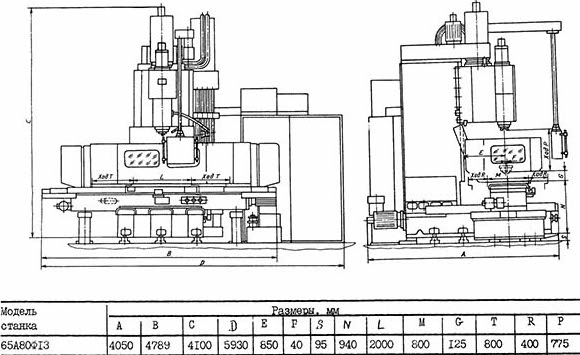
\includegraphics[width=.90\linewidth]{spr_65a80_1.jpg}
    \caption{габаритные размеры рабочего поля}
    \label{subfig:65a80a}
  \end{subfigure}%
  \begin{subfigure}[b]{.50\textwidth}
    \centering
    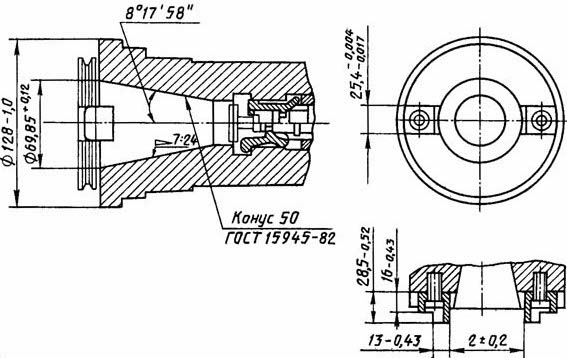
\includegraphics[width=.90\linewidth]{spr_2206vmf4_2.jpg}
    \caption{посадочные и присоединительные базы}
    \label{subfig:65a80b}
  \end{subfigure}%
  \caption{Посадочные и присоединительные размеры станка 65А80}
  \label{fig:65a80}
\end{figure}

% \newpage
\subsection{Выбор и обоснование схемы базирования}

Базирование осуществляется по схеме, представленной на рис.~\ref{fig:b045}

\begin{figure}[H]
	\centering
	   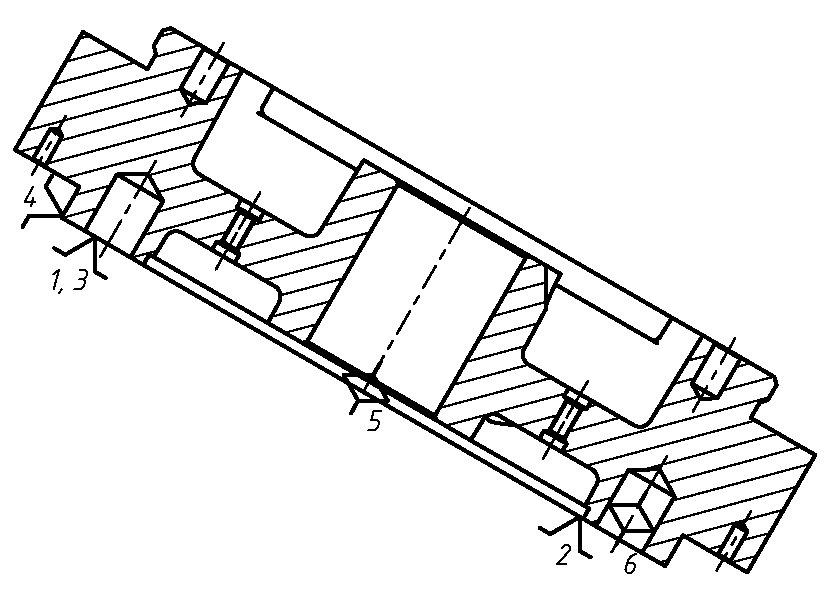
\includegraphics[width=0.7\textwidth]{bases_045.pdf}
	   \caption{Схема базирования на операции 045}
	   \label{fig:b045}
	   1, 2, 3 --- установочная база, \\
	   4, 5 --- направляющая база, \\
	   6 --- опорная база
\end{figure}

\subsection{Выбор и обоснование последовательности и содержания переходов}

На операции 045 осуществляется обработка паза, расположенных под углом к торцу детали. Деталь установлена в специальном приспособлении под наклоном. Обработка паза производится за один проход концевой фрезой, радиус которой совпадает с радиусом скруглений паза. Последовательность обработки приведена в табл.~\ref{tab:045}.

\begin{table}[H]
  \setlength{\tabulinesep}{1.2ex}
  \begin{longtabu} to \textwidth { | X[7,l,p] | }
    \caption{Содержание основных переходов операции 045} \label{tab:045} \\
  
      \hline 
      \multicolumn{1}{|c|}{\linespread{1.1} \bfseries{\small Содержание переходов}} \\ \hline 
    \endfirsthead
  
      \multicolumn{1}{l}{{\itshape Продолжение таблицы \thetable{}}} \\ \hline 
      \multicolumn{1}{|c|}{\linespread{1.1} \bfseries{\small Содержание переходов}} \\ \hline
    \endhead
  
      \hline
    \endfoot

      -- Фрезеровать паз \circled{34}, выдерживая размер $20 \times \ang{60}$ и ширину $50$ \\ \hline

  \end{longtabu}
\end{table}

\subsection{Выбор и характеристика режущего инструмента}

Для фрезерования паза \circled{34} выбрана концевая фреза 1-25 ГОСТ~Р 50572-93. Материал режущей части фрезы --- быстрорежущая сталь Р6М5 \cite[прил.~4]{guzeev:rr}.

\subsection{Расчёт режимов и сил резания}

Расчёт ведётся табличным методом по методике, приведённой в \cite{guzeev:rr}.

Обработка происходит за один рабочий ход.

Ширину фрезерования $B$ измеряют в направлении, параллельном оси фрезы, а глубину резания $t$ --- в направлении, перпендикулярном оси фрезы.

При выбранной схеме обработки $ B_\text{max} = \SI{37,5}{\milli\meter} $, $ t_\text{max} = \SI{15,3}{\milli\meter} $.

Табличное значение подачи корректируют по формуле:
\begin{equation}
  S_z = {S_z}_\text{т} \; K_{S_\text{м}} \; K_{S_\text{н}} \; K_{S_\text{z}} \; K_{S_\text{l}}
\end{equation}

$ {S_z}_\text{т} = \SI{0,09}{\milli\meter\per\tooth} $ \cite[карта 81]{guzeev:rr} \par
$ K_{S_\text{м}} = K_{S_\text{н}} = 1,0 $ \par
$ K_{S_\text{z}} = 0,60 $ \par
$ K_{S_\text{l}} = 0,85 $ \cite[карта 82]{guzeev:rr}
\begin{equation*}
  S_z = 0,09 \cdot 1,00 \cdot 0,60 \cdot 0,85 = \SI{0,05}{\milli\meter\per\tooth}
\end{equation*}

Полученное значение сравнивают с максимально допустимым при заданной шероховатости поверхности. Для получения шероховатости Ra~6,3 при фрезеровании фрезой $\diameter 25$ с шестью зубьями $ S_z^\text{max} = \SI{0,07}{\milli\meter\per\tooth} $. Окончательно выбирается меньшее значение.

Подача при врезании должна быть снижена на \SI{30}{\percent}.

Табличное значение скорости резания корректируют по формуле:
\begin{equation}
  V = {V}_\text{т} \; K_{V_\text{о}} \; K_{V_\text{м}} \; K_{V_\text{н}} \; K_{V_\text{T}} \; K_{V_\text{B}} \; K_{V_\text{п}} \; K_{V_\text{ж}}
\end{equation}

$ {V}_\text{т} = \SI{18}{\meter\per\minute} $ \cite[карта 87]{guzeev:rr} \par
$ K_{V_\text{o}} = K_{V_\text{м}} = K_{V_\text{н}} = K_{V_\text{T}} = K_{V_\text{ж}} = 1,00 $ \par
$ K_{V_\text{B}} = 0,93 $ \par
$ K_{V_\text{п}} = 0,80 $ \cite[карта 85]{guzeev:rr}
\begin{gather*}
  V = 18 \cdot 1,00 \cdot 0,93 \cdot 0,80 = \SI{13,4}{\meter\per\minute} \\
  n = \frac{1000 V}{\pi D} \frac{1000 \cdot 13,4}{\pi \cdot 25} = \SI{170,6}{\rev\per\minute} \\
  S_m = S_z z n = 0,05 \cdot 6 \cdot 170,6 = \SI{51,2}{\milli\meter\per\minute}
\end{gather*}

Станок позволяет регулировать обороты шпинделя и подачи бесступенчато. Фактические режимы резания округляют до значений из стандартных рядов предпочтительных чисел в меньшую сторону: $n_\text{ф} = \SI{160}{\rev\per\minute}$, ${S_\text{м}}_\text{ф} = \SI{50}{\milli\meter\per\minute}$.

Фактическая скорость резания:
\begin{equation*}
  V_\text{ф} = \frac{\pi D n_\text{ф}}{1000} = \frac{\pi \cdot 25 \cdot 160}{1000} = \SI{12,6}{\meter\per\minute}
\end{equation*}

Табличное значение мощности резания корректируют по формуле:
\begin{equation}
  N = {N}_\text{т} \; K_{N_\text{о}} \; K_{N_\text{м}} \; K_{N_\text{н}} \; K_{N_\text{T}} \; K_{N_\text{B}} \; K_{N_\text{п}} \; K_{N_\text{ж}}
\end{equation}

$ {N}_\text{т} = \SI{1,38}{\kilo\watt} $ \cite[карта 87]{guzeev:rr} \par
$ K_{N_\text{o}} = K_{N_\text{м}} = K_{N_\text{н}} = K_{N_\text{T}} = K_{N_\text{ж}} = 1,00 $ \par
$ K_{N_\text{B}} = 0,93 $ \par
$ K_{N_\text{п}} = 0,80 $ \cite[карта 85]{guzeev:rr}
\begin{equation*}
  V = 1,38 \cdot 1,00 \cdot 0,93 \cdot 0,80 = \SI{1,03}{\kilo\watt}
\end{equation*}

Составляющие силы резания корректируют по формуле:
\begin{equation}
  P = {P}_\text{т} \; K_{P_\text{о}} \; K_{P_\text{м}} \; K_{P_\text{z}} \; K_{P_\text{B}}
\end{equation}

$ {P_y}_\text{т} = \SI{950}{\newton} $ \par
$ {P_z}_\text{т} = \SI{2875}{\newton} $ \cite[карта 88]{guzeev:rr} \par
$ K_{P_\text{o}} = 0,90 $ \par
$ K_{P_\text{м}} = 1,00 $ \par
$ K_{P_\text{z}} = 1,50 $ \par
$ K_{P_\text{B}} = 2,00 $ \cite[карта 88]{guzeev:rr}
\begin{gather*}
  {P_y}_\text{т} = 950 \cdot 1,00 \cdot 0,90 \cdot 1,50 \cdot 2,00 = \SI{2565}{\newton} \\
  {P_z}_\text{т} = 2875 \cdot 1,00 \cdot 0,90 \cdot 1,50 \cdot 2,00 = \SI{7763}{\newton}
\end{gather*}

Основное время обработки паза рассчитывается по формуле:
\begin{gather*}
  t_o = \frac{l}{S_\text{м}} + \frac{l_\text{вр}}{S_\text{м}^\text{вр}}  \\
  S_\text{м}^\text{вр} = S_\text{м} - \SI{30}{\percent}
\end{gather*}
где $l$ --- длина обработки, $\left[\si{\rev\per\minute}\right]$ \par
$l_\text{вр}$ --- длина движения врезания, $\left[\si{\rev\per\minute}\right]$
\begin{gather*}
  S_\text{м}^\text{вр} = 0,7 \cdot 50 = \SI{35}{\rev\per\minute} \\
  l = \SI{25}{\milli\meter} \\
  l^\text{вр} = \SI{15}{\milli\meter} \\
  t_o = \frac{25}{50} + \frac{15}{35} = \SI{0,93}{\minute}
\end{gather*}

Полученные значения параметров режимов резания сведены в табл.~\ref{tab:rr045}.\begin{table}[H]
  \setlength{\tabulinesep}{1.2ex}
  \begin{longtabu} to \textwidth { | S[table-format=2.1] | S[table-format=2] | S[table-format=3] | S[table-format=2.1] | S[table-format=1.2] | }
    \caption{Режимы резания для переходов операции 045} \label{tab:rr045} \\
  
      \hline 
      \multicolumn{1}{|c|}{$t$, \si{\milli\meter}} & 
      \multicolumn{1}{|c|}{$S_\text{м}$, \si{\milli\meter\per\minute}} & 
      \multicolumn{1}{|c|}{$n$, \si{\rev\per\minute}} & 
      \multicolumn{1}{|c|}{$V$, \si{\meter\per\minute}} & 
      \multicolumn{1}{|c|}{$t_o$, \si{\minute}} \\ \hline 
    \endfirsthead
  
      \multicolumn{5}{l}{{\itshape Продолжение таблицы \thetable{}}} \\ \hline 
      \multicolumn{1}{|c|}{$t$, \si{\milli\meter}} & 
      \multicolumn{1}{|c|}{$S_\text{м}$, \si{\milli\meter\per\minute}} & 
      \multicolumn{1}{|c|}{$n$, \si{\rev\per\minute}} & 
      \multicolumn{1}{|c|}{$V$, \si{\meter\per\minute}} & 
      \multicolumn{1}{|c|}{$t_o$, \si{\minute}} \\ \hline 
    \endhead
  
      \hline
    \endfoot

    15,3 & 50  & 160  & 12,6  & 0,93 \\ \hline


  \end{longtabu}
\end{table}

\subsection{Техническое нормирование}

Под техническим нормированием подразумевается определение технически обоснованной нормы времени на выполнение операции.

Штучное время $t_\text{шт}$ рассчитывается по формуле:
\begin{equation*}
  t_\text{шт} = t_\text{о} + t_\text{в} + t_\text{обс}
\end{equation*}
где $t_\text{о}$ --- основное время операции \par
$t_\text{в}$ --- вспомогательное время \par
$t_\text{обс}$ --- время на обслуживание рабочего места

Вспомогательное время рассчитывается по формуле:
\begin{equation*}
  t_\text{в} = t_\text{уст} + t_\text{в. о.} + t_\text{изм}^\text{шт}
\end{equation*}
где $t_\text{уст}$ --- время установки заготовки \par
$t_\text{в. о.}$ --- время, связанное с выполнением операции \par
$t_\text{изм}^\text{шт}$ --- время на измерения, приведённое к одной детали

Время установки рассчитывается по формуле:
\begin{equation*}
  t_\text{уст} = a \cdot Q^x
\end{equation*}
где $a$, $x$ --- коэффициенты, зависящие от схемы закрепления \par
$Q$ --- вес заготовки $\left[\si{\kilo\gram}\right]$

Для установки в специальном приспособлении по отверстию с креплением гайкой или винтом ключом $ a = 0,26 $, $ x = 1,0 $ \cite[прил.~3]{malzen:normirovanie}.
\begin{equation*}
  t_\text{уст} = 0,26 \cdot 250,8^{0,22} = \SI{0,88}{\minute}
\end{equation*}

Время, связанное с выполнением операции \cite[прил.~4]{malzen:normirovanie}: \\
Включение станка: $\SI{0,02}{\minute}$; \\
Подвод инструмента: $\SI{0,02}{\minute}$; \\
Отвод инструмента: $\SI{0,02}{\minute}$; \\
Выключение станка: $\SI{0,02}{\minute}$. \\
\begin{equation*}
  t_\text{в. о.} = 0,02 + 0,02 + 0,02 + 0,02 = \SI{0,08}{\minute}
\end{equation*}

Время на измерения рассчитывается по формуле:
\begin{equation*}
  t_\text{изм} = \sum k D_\text{изм}^z L_\text{изм}^u
\end{equation*}
где $k$, $z$, $u$ --- коэффициенты, зависящие от способа измерения \par
$D_\text{изм}$, $L_\text{изм}$ --- размеры контролируемой поверхности $[\si{\milli\meter}$

Для контроля размера угла фасонным шаблоном простого профиля с точностью \SIrange{0,15}{0,25}{\milli\meter} $ k = 0,0113 $, $ u = 0 $, $ z = 0,368 $ \cite[прил.~5]{malzen:normirovanie}.
\begin{equation*}
  t_\text{изм} = 0,0113 \cdot 50^{0,368} = \SI{0,05}{\minute}
\end{equation*}

При выборочном время измерения приводится к одной детали по формуле:
\begin{equation*}
  t_\text{изм}^\text{шт} = \frac{k}{100} \; t_\text{изм}
\end{equation*}
где $k$ --- число контрольных измерений на 100 деталей $[\%]$

Для фрезерования плоскостей $ k = \SI{10}{\percent} $.
\begin{equation*}
  t_\text{изм}^\text{шт} = \frac{10}{100} \cdot 0,05 = \SI{0,01}{\minute}
\end{equation*}

\begin{equation*}
  t_\text{в} = 0,88 + 0,08 + 0,01 = \SI{0,97}{\minute}
\end{equation*}

Время обслуживания рабочего места определяется в процентах от суммы основного и вспомогательного: 
\begin{equation*}
  t_\text{обс} = \frac{k}{100} \; (t_\text{о} + t_\text{в})
\end{equation*}
где $k$ --- коэффициент, зависящий от вида оборудования $[\%]$

Для обработки на фрезерных станках с длиной стола \SIrange{700}{1500}{\milli\meter} $ k = \SI{4,5}{\percent} $ \cite[прил.~5]{malzen:normirovanie}.

\begin{equation*}
  t_\text{обс} = \frac{4,5}{100} \; (0,93 + 0,97) = \SI{0,09}{\minute}
\end{equation*}

\begin{equation*}
  t_\text{шт} = 0,93 + 0,97 + 0,09 = \SI{1,99}{\minute}
\end{equation*}

Штучно-калькуляционное время $t_\text{шт}^\text{к}$ включает в себя подготовительно-заключительное время на операцию. Его можно приближённо рассчитать по формуле: 
\begin{equation*}
  t_\text{шт}^\text{к} = \varphi_\text{k} t_\text{шт}
\end{equation*}
где $\varphi_\text{k}$ --- коэффициент, зависящий от типа станка

Для обработки на фрезерных станках $ \varphi_\text{k} = 1,75 $ \cite[прил.~7]{malzen:normirovanie}.
\begin{equation*}
  t_\text{шт}^\text{к} = 1,75 \cdot 1,99 = \SI{3,48}{\minute}
\end{equation*}


\subsection{Выбор методов и средств операционного контроля}
Для контроля выдерживаемого угла используется фасонный шаблон.


\chapter{Расчёт и проектирование станочных приспособлений}

\section{Приспособление для сверлильной операции с ЧПУ}

\subsection{Характеристика и описание принципа работы приспособления}

Спроектированное приспособление --- специальное, одноместное, с ручным приводом. Предназначено для установки и закрепления заготовки на поворотном столе станка на сверлильной операции с ЧПУ.

Заготовка устанавливается на установочные элементы, закреплённые на плите приспособления и закрепляется с помощью быстросъёмной шайбы, что позволяет ускорить процесс установки. Усилие закрепления создаётся вручную гайкой М20.

Установочные элементы приспособления --- три плоские опоры, цилиндрический палец $\diameter 125$ и срезанный палец $\diameter 25$. Технологические базы детали выбраны так, чтобы обеспечить их совпадение с измерительными, в соответствии с принципом совмещения баз.

Приспособление базируется на столе станка при помощи круглых штифтов, один из которых ориентирует приспособление по центральному отверстию стола станка, обеспечивая совпадение оси приспособления с осью вращения стола, а второй --- по Т-образному пазу стола, предотвращая поворот приспособления относительно стола. Приспособление закрепляется на столе четырьмя болтами для Т-образных пазов.

\subsection{Силовой расчёт приспособления}

Приложенная сила закрепления должна исключить возможность отрыва, сдвига или проворота заготовки под действием сил резания на протяжении всего процесса обработки. Сущность силового расчёта заключается в том, чтобы определить силу закрепления, которая обеспечит равновесие заготовки под действием всех приложенных к ней внешних сил: сил резания, закрепления, реакции опор и сил трения.

Для силового расчёта необходимо составить расчётную схему, на которой обозначены внешние силы, действующие на заготовку.

\begin{figure}[H]
	\centering
	   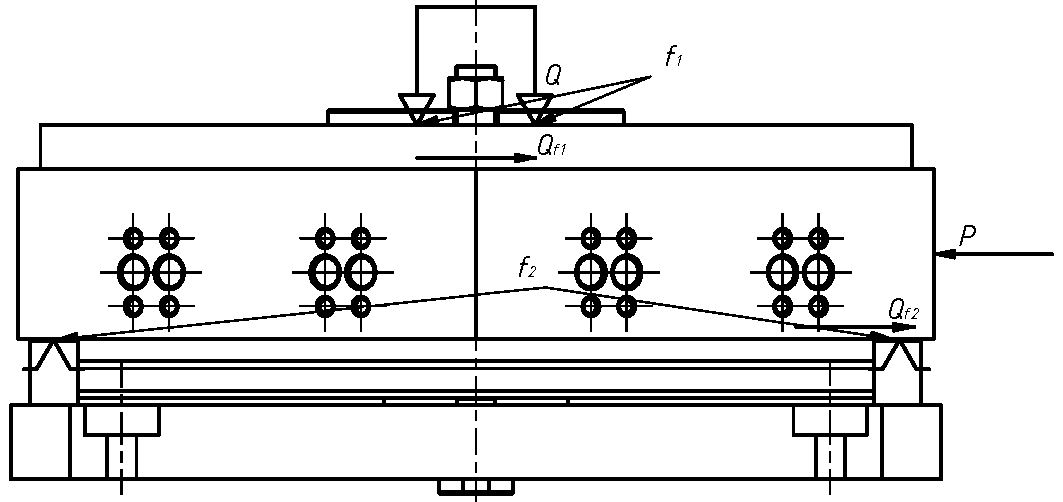
\includegraphics[width=0.85\textwidth]{force_040.pdf}
	   \caption{Расчётная схема для силового расчёта приспособления для операции 040}
	   \label{fig:f040}
\end{figure}

При данной расчётной схеме сила закрепления должна удовлетворять обоим условиям:
\begin{gather}
  Q \geq \frac{K \; P}{f_1 + f_2} \\
  Q \geq \frac{K \; P \; r_P}{f_1 \; r_1 + f_2 \; r_2}
\end{gather}
где $K$ --- коэффициент запаса \par
$P$ --- сила резания, возникающая при обработке $\left[\si{\newton}\right]$ \par
$f_1$, $f_2$ --- коэффициенты трения между поверхностью заготовки и установочными и зажимными элементами приспособления \par
$r_P$, $r_1$, $r_2$ --- плечи приложения соответствующих сил $\left[\si{\milli\meter}\right]$

Силы резания в процессе обработки изменяются, поэтому для обеспечения надёжности закрепления силу зажима рассчитывают с учётом коэффициента запаса. Он рассчитывается по формуле:
\begin{equation}
  K = K_0 \; K_1 \; K_2 \; K_3 \; K_4 \; K_5 \; K_6
\end{equation}
где $K_0 = 1,5$ --- гарантированный коэффициент запаса \par
$K_1 = 1$ --- коэффициент, учитывающий увеличение силы резания из-за случайных неровностей на заготовке\par
$K_2 = 1$ --- коэффициент, учитывающий увеличение силы резания из-за затупления инструмента \par
$K_3 = 1$ --- коэффициент, учитывающий увеличение силы резания при прерывистом резании \par
$K_4 = 1,2$ --- коэффициент, учитывающий непостоянство усилия зажима \par
$K_5 = 1,2$ --- коэффициент, учитывающий удобство расположения рукоятки ручного зажимного устройства \par
$K_6 = 1,1$ --- коэффициент, учитывающий неопределённости из-за неровностей места контакта заготовки с опорными элементами, имеющими ограниченную опорную поверхность

Значения коэффициентов выбраны по рекомендациям \cite[разд.~4.1]{tarabarin:pto}.
\begin{equation*}
  K = 1,5 \cdot 1 \cdot 1 \cdot 1 \cdot 1,2 \cdot 1,2 \cdot 1,1 = 2,38
\end{equation*}
Принимают коэффициент запаса $K \geq 2,5$.

В соответствии с условиями контакта установочных и зажимных элементов с заготовкой, выбраны коэффициенты $ f_1 = f_2 = 0,16 $ \cite[с.~85]{kosilova:stm2}.

Максимальную силу, действующую в процессе обработки, оказывает сверло $\diameter 18,5$ на переходе T01. Это осевая сила $ P = \SI{4345}{\newton} $.
\begin{gather*}
  Q \geq \frac{2,5 \cdot 4345}{0,16 + 0,16} = \SI{33945}{\newton} \\
  Q \geq \frac{2,5 \cdot 4345 \cdot 89}{0,16 \cdot 75 + 0,16 \cdot 330} = \SI{14919}{\newton}
\end{gather*}
Выбирается наибольшее из полученных значений. $ Q = \SI{33945}{\newton} $

Закрепление осуществляется гайкой. При известной силе закрепления номинальный диаметр винта $d$ вычисляют по формуле:
\begin{equation}
  d = 1,4 \; \sqrt{\frac{Q}{\left[\sigma\right]_\text{р}}}
\end{equation}
где $\left[\sigma\right]_\text{р}$ --- допустимое напряжение растяжения материала винта $\left[\si{\mega\pascal}\right]$

Для Стали 45 $ \left[\sigma\right]_\text{р} = \SI{200}{\mega\pascal} $.
\begin{equation*}
  d = 1,4 \; \sqrt{\frac{33945}{200}} = \SI{18,2}{\milli\meter}
\end{equation*}
Назначена резьба M20.

Необходимый момент на гайке рассчитывается по формуле: \cite[с.~87]{kosilova:stm2}
\begin{equation}
  M_\text{кр} = 0,2 \; Q d_2
\end{equation}
где $d_2$ --- средний диаметр резьбы $\left[\si{\milli\meter}\right]$

Для резьбы M20 $ d_2 = \SI{18,376}{\milli\meter} $.
\begin{equation*}
  M_\text{кр} = 0,2 \cdot 33945 \cdot 18,379 = \SI{124756}{\newton\milli\meter} = \SI{124,8}{\newton\meter}
\end{equation*}

В приспособлениях с ручным приводом усилие на конце рукоятки при закреплении не должно превышать $\SI{160}{\newton}$. Необходимая для выполнения этого условия длина рукоятки $L$ определяется по формуле:
\begin{equation}
  L = \frac{M_\text{кр}}{P_\text{max}}
\end{equation}
\begin{equation*}
  L = \frac{124,8}{160} = \SI{0,78}{\meter}
\end{equation*}

\subsection{Прочностной расчёт приспособления}

При проектировании приспособления выполняют расчёт на прочность «слабого звена» --- наиболее нагруженного элемента конструкции.

Сущность прочностного расчёта заключается в определении действующих на «слабое звено» напряжений и сравнении их с допускаемыми.

В проектируемом приспособлении «слабым звеном», наиболее вероятно, окажется шпилька, с помощью которой осуществляется закрепление. Произведён её расчёт на разрыв по внутреннему диаметру резьбы.

Условие прочности можно определить как: \cite[форм.~14.6]{ryahovskiy:dm}
\begin{equation}
  \sigma = \frac{4 \; Q}{\pi d_3^2} \leq \left[ \sigma \right]_p
\end{equation}
где $Q$ --- сила, растягивающая болт $\left[\si{\newton}\right]$ \par
$d_3$ --- внутренний диаметр резьбы $\left[\si{\milli\meter}\right]$ \par
$\left[ \sigma \right]_p$ --- допускаемое напряжение $\left[\si{\mega\pascal}\right]$

Для резьбы M20 $ d_3 = \SI{16,933}{\milli\meter} $.
\begin{equation*}
  \sigma = \frac{4 \; 33945}{\pi \cdot 16,933^2} = \SI{150,7}{\mega\pascal}
\end{equation*}

Для Стали 45 $ \left[\sigma\right]_\text{р} = \SI{200}{\mega\pascal} $
\begin{equation*}
  \SI{150,7}{\mega\pascal} < \SI{200}{\mega\pascal}
\end{equation*}

Условие прочности выполняется, значит прочность «слабого звена» обеспечивается.

\subsection{Расчёт приспособления на точность}

Диаметры отверстий и размеры резьбы обеспечиваются инструментами и не зависят от способа установки. Расстояния между осями отверстий определяются точностью позиционирования станка и также не зависят от установки. Для перечисленных размеров погрешность установки равна нулю. Расчётная схема представлена на рис.~\ref{fig:d040}

\begin{figure}[H]
	\centering
	   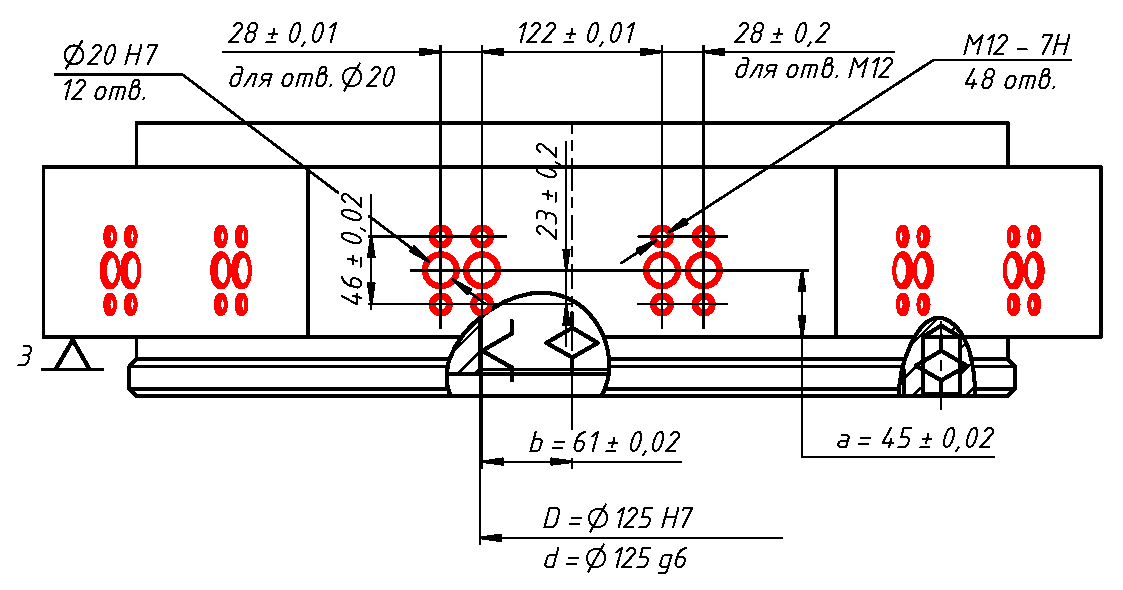
\includegraphics[width=0.75\textwidth]{dim_040.pdf}
	   \caption{Расчётная схема для расчёта на точность приспособления для операции 040}
	   \label{fig:d040}
\end{figure}

Размерами, определяющими положение группы отверстий относительно баз заготовки, будут $ a = 45 \pm 0,02 $ и $ b = 61 \pm 0,02 $.

\subparagraph{Погрешность базирования} \

Для размера $a$ измерительная база совпадает с технологической. Для него погрешность базирования $ \varepsilon_{\text{б} \, a} = 0 $.

Погрешность базирования размера $b$ определяется по формуле: \cite[с.~60]{tarabarin:pto}
\begin{equation}
  \varepsilon_{\text{б}} = \frac{S}{2} + \frac{\text{TD}}{2}
\end{equation}
где $S$ --- минимальный зазор между базовым отверстием и пальцем $\left[\si{\micro\meter}\right]$ \par
$\text{TD}$ --- допуск на размер отверстия $\left[\si{\micro\meter}\right]$

\begin{equation*}
  \varepsilon_{\text{б} \, b} = \frac{14}{2} + \frac{40}{2} = \SI{27}{\micro\meter}
\end{equation*}

\subparagraph{Погрешность закрепления} \

Погрешность закрепления вызывается непостоянством силы закрепления. Погрешность закрепления влияет только на размеры, измеряемые в направлении действия силы закрепления. Для размера $b$ погрешность закрепления $ \varepsilon_{\text{закр} \, b} = 0 $.

Погрешность закрепления размера $a$ определяется по формуле: \cite[с.~64]{tarabarin:pto}
\begin{equation}
  \varepsilon_{\text{закр}} = y_\text{max} - y_\text{min} = C_\text{max} \; Q_\text{max}^n - C_\text{min} \; Q_\text{min}^n
\end{equation}
где $C$ --- коэффициент, характеризующий условия контакта \par
$n$ --- эмпирический коэффициент \par
$Q$ --- сила, приходящаяся на опору $\left[\si{\newton}\right]$

Для плоских опор приняты коэффициенты $ C = 0,6 \pm 1 \; \% $, $ n = 0,6 $. Сила закрепления $ Q = \frac{33945}{3} \pm 10 \; \% \; \si{\newton} $. 
\begin{equation*}
  \varepsilon_{\text{закр} \, b} = 0,606 \cdot \left( \frac{37339,5}{3} \right)^{0,6} - 0,594 \cdot \left( \frac{30550,5}{3} \right)^{0,6} = \SI{20}{\micro\meter}
\end{equation*}

\newpage
\subparagraph{Погрешность приспособления} \

Погрешность приспособления складывается из трёх составляющих: погрешности изготовления элементов приспособления, погрешности, вызванной износом установочных элементов и погрешности установки приспособления на станок. Приспособление установлено на станке неизменно на протяжении изготовления всей партии деталей, а установочные элементы не меняются, поэтому первая и третья составляющая приравниваются к нулю. Погрешность, вызванная износом установочных элементов, равна величине износа.
\begin{equation}
  \varepsilon_{\text{и}} = u = \beta_2 \; N
\end{equation}
где $\beta_2$ --- эмпирический коэффициент \par
$N$ --- число установок детали на приспособление

Число установок детали принято равным программе запуска, $ N = \SI{258}{\pcs} $. Для плоских опор $ \beta_2 = \numrange{0,04}{0,08} $; для цилиндрических пальцев $ \beta_2 = \numrange{0,005}{0,01} $.
\begin{gather*}
  \varepsilon_{\text{и} \, a} = 0,06 \cdot 258 = \SI{15,5}{\micro\meter} \\
  \varepsilon_{\text{и} \, b} = 0,007 \cdot 258 = \SI{1,8}{\micro\meter}
\end{gather*}

\subparagraph{Погрешность установки} \

Суммарная погрешность установки рассчитывается по формуле:
\begin{equation}
  \varepsilon = \sqrt{\varepsilon_\text{б}^2 + \varepsilon_\text{закр}^2 + 3 \; \varepsilon_\text{и}^2}
\end{equation}

Тогда:
\begin{gather*}
  \varepsilon_a = \sqrt{0 + 20^2 + 3 \cdot 15,5^2} = \SI{33,5}{\micro\meter} < \SI{40}{\micro\meter} \\
  \varepsilon_b = \sqrt{27^2 + 0 + 3 \cdot 1,8^2} = \SI{27,2}{\micro\meter} < \SI{40}{\micro\meter}
\end{gather*}
Погрешности установки всех размеров меньше, чем их допуски, значит необходимую точность возможно обеспечить, используя спроектированное приспособление.


\section{Приспособление для фрезерной операции}

\subsection{Характеристика и описание принципа работы приспособления}

Спроектированное приспособление --- специальное, одноместное, с ручным приводом. Предназначено для установки и закрепления заготовки под наклоном на столе фрезерного станка для фрезеровки паза под углом.

Заготовка устанавливается на установочные элементы, закреплённые на плите приспособления и закрепляется с помощью быстросъёмной шайбы, что позволяет ускорить процесс установки. Усилие закрепления создаётся вручную гайкой М20.

Установочные элементы приспособления --- обработанная плоскость плиты, выточка $\diameter 590$ и срезанный палец $\diameter 45$.

Приспособление закрепляется на столе станка четырьмя болтами для Т-образных пазов.

Наклон плит приспособления относительно друг друга осуществляется с помощью элементов универсальной станочной оснастки --- угловых опор. Опоры базируются на основании по цилиндрическим штифтам, закрепляется болтом. На опорах таким же образом установлена наклонная плита, на которую устанавливается заготовка.

\subsection{Силовой расчёт приспособления}

Приложенная сила закрепления должна исключить возможность отрыва, сдвига или проворота заготовки под действием сил резания на протяжении всего процесса обработки. Сущность силового расчёта заключается в том, чтобы определить силу закрепления, которая обеспечит равновесие заготовки под действием всех приложенных к ней внешних сил: сил резания, закрепления, реакции опор и сил трения.

Для силового расчёта необходимо составить расчётную схему, на которой обозначены внешние силы, действующие на заготовку.

\begin{figure}[H]
	\centering
	   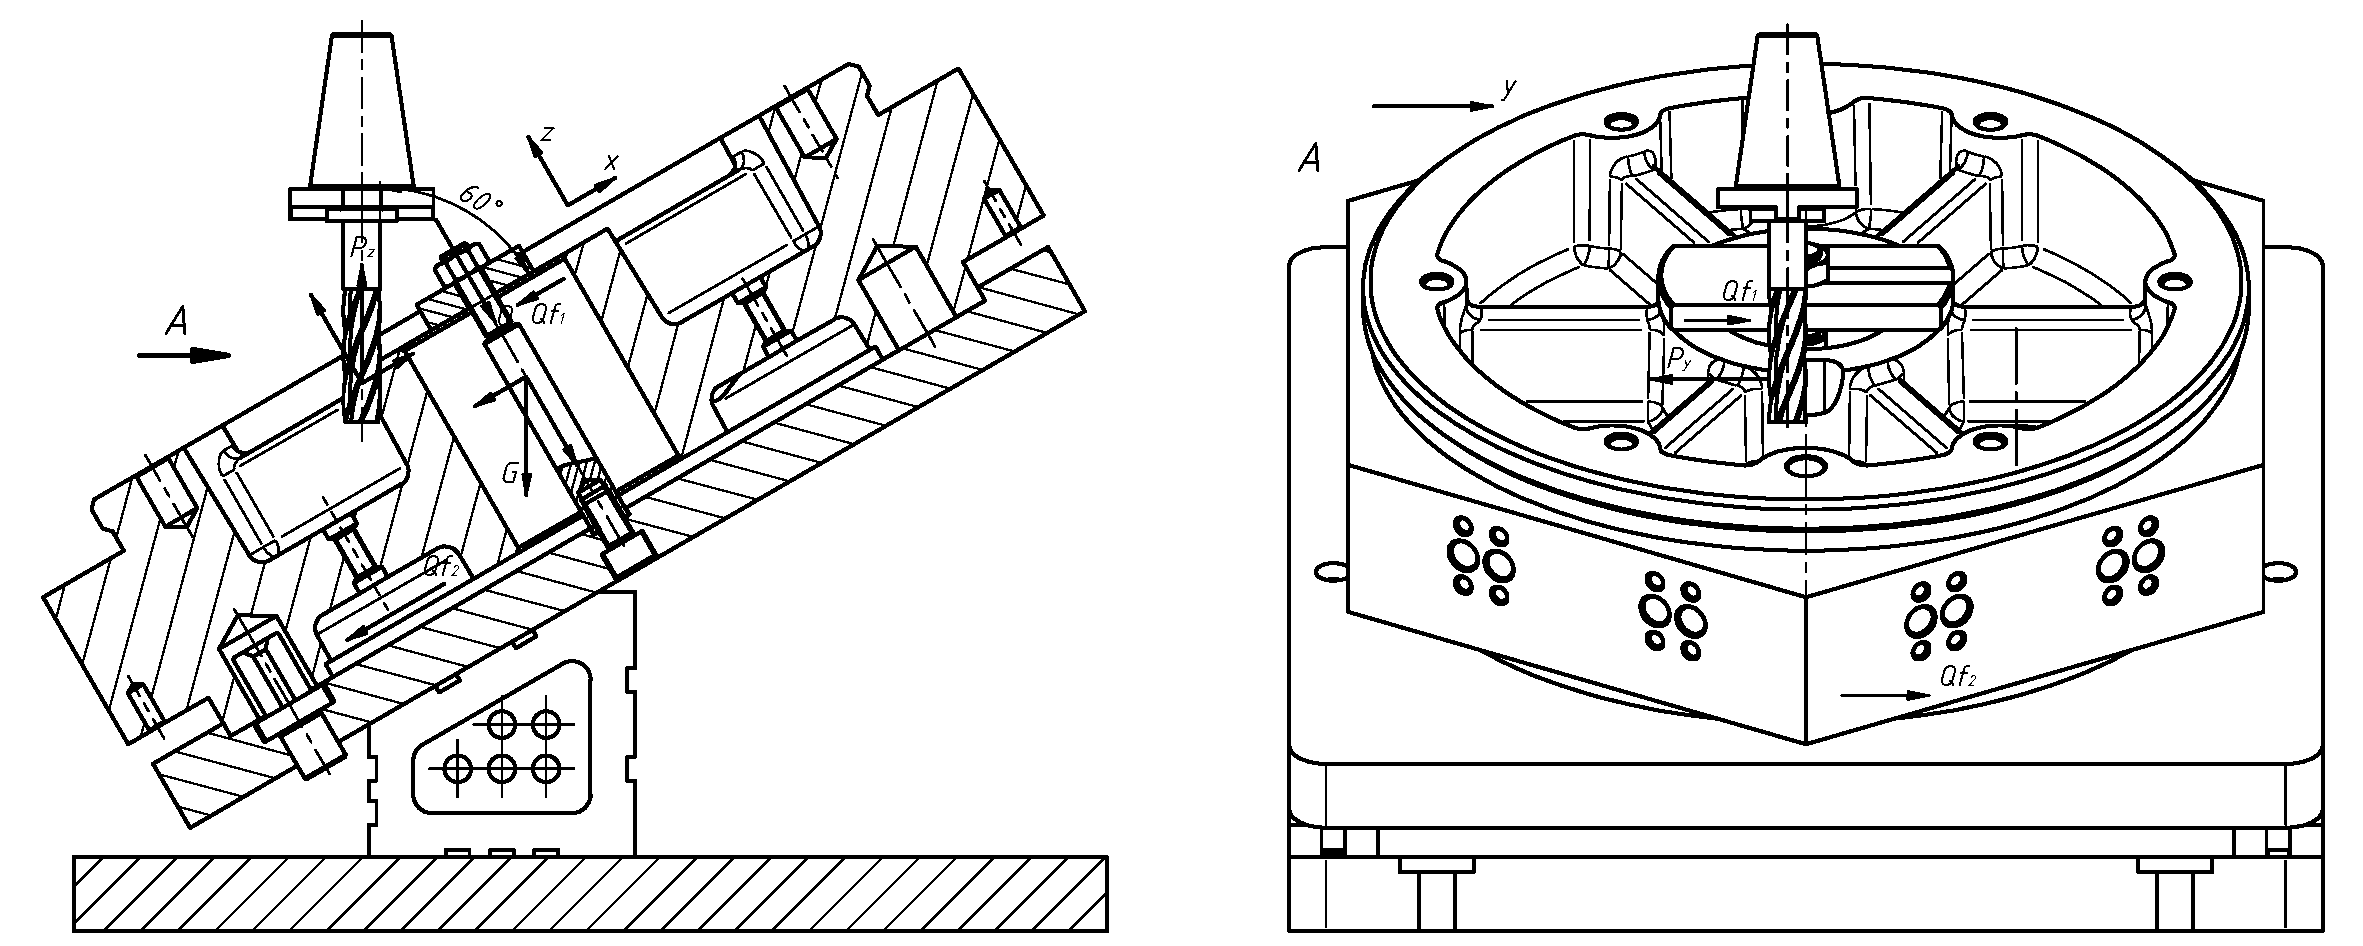
\includegraphics[width=0.9\textwidth]{force_045.pdf}
	   \caption{Расчётная схема для силового расчёта приспособления для операции 045}
	   \label{fig:f045}
\end{figure}

При данной расчётной схеме сила закрепления должна удовлетворять каждому из следующих условий:
\begin{gather}
  Q \geq K \; \frac{P_z \; \cos{\ang{60}} - G \; \cos{\ang{60}}}{f_1 + f_2} \\
  Q \geq K \; ( P_z \; \sin{\ang{60}} - G \; \sin{\ang{60}} ) \\
  Q \geq K \; \frac{P_y}{f_1 + f_2}
\end{gather}
где $K$ --- коэффициент запаса \par
$P_z$, $P_y$ --- соответствующие компоненты силы резания, возникающей при обработке $\left[\si{\newton}\right]$ \par
$G$ --- вес заготовки $\left[\si{\newton}\right]$ \par
$f_1$, $f_2$ --- коэффициенты трения между поверхностью заготовки и установочными и зажимными элементами приспособления

Силы резания в процессе обработки изменяются, поэтому для обеспечения надёжности закрепления силу зажима рассчитывают с учётом коэффициента запаса. Он рассчитывается по формуле:
\begin{equation*}
  K = K_0 \; K_1 \; K_2 \; K_3 \; K_4 \; K_5 \; K_6
\end{equation*}
где $K_0 = 1,5$ --- гарантированный коэффициент запаса \par
$K_1 = 1$ --- коэффициент, учитывающий увеличение силы резания из-за случайных неровностей на заготовке\par
$K_2 = 1$ --- коэффициент, учитывающий увеличение силы резания из-за затупления инструмента \par
$K_3 = 1$ --- коэффициент, учитывающий увеличение силы резания при прерывистом резании \par
$K_4 = 1,2$ --- коэффициент, учитывающий непостоянство усилия зажима \par
$K_5 = 1,2$ --- коэффициент, учитывающий удобство расположения рукоятки ручного зажимного устройства \par
$K_6 = 1,1$ --- коэффициент, учитывающий неопределённости из-за неровностей места контакта заготовки с опорными элементами, имеющими ограниченную опорную поверхность

Значения коэффициентов выбраны по рекомендациям \cite[разд.~4.1]{tarabarin:pto}.
\begin{equation*}
  K = 1,5 \cdot 1 \cdot 1 \cdot 1 \cdot 1,2 \cdot 1,2 \cdot 1,1 = 2,38
\end{equation*}
Принимают коэффициент запаса $K \geq 2,5$.

В соответствии с условиями контакта установочных и зажимных элементов с заготовкой, выбраны коэффициенты $ f_1 = f_2 = 0,16 $ \cite[с.~85]{kosilova:stm2}.

Силы, возникающие в процессе обработки: $ P_y = \SI{950}{\newton} $, $ P_z = \SI{2875}{\newton} $. Вес заготовки: $ G = \SI{2458}{\newton} $
\begin{gather*}
  Q \geq 2,5 \; \frac{2875 \; \cos{\ang{60}} - 2458 \; \cos{\ang{60}}}{0,16 + 0,16} = \SI{1630}{\newton} \\
  Q \geq 2,5 \; ( 2875 \; \sin{\ang{60}} - 2458 \; \sin{\ang{60}} ) = \SI{903}{\newton} \\
  Q \geq 2,5 \; \frac{950}{0,16 + 0,16} = \SI{7422}{\newton}
\end{gather*}
Выбирается наибольшее из полученных значений. $ Q = \SI{7422}{\newton} $

Закрепление осуществляется гайкой. При известной силе закрепления номинальный диаметр винта $d$ вычисляют по формуле:
\begin{equation*}
  d = 1,4 \; \sqrt{\frac{Q}{\left[\sigma\right]_\text{р}}}
\end{equation*}
где $\left[\sigma\right]_\text{р}$ --- допустимое напряжение растяжения материала винта $\left[\si{\mega\pascal}\right]$

Для Стали 45 $ \left[\sigma\right]_\text{р} = \SI{200}{\mega\pascal} $.
\begin{equation*}
  d = 1,4 \; \sqrt{\frac{7421}{200}} = \SI{7,6}{\milli\meter}
\end{equation*}
Назначена резьба M20.

Необходимый момент на гайке рассчитывается по формуле: \cite[с.~87]{kosilova:stm2}
\begin{equation*}
  M_\text{кр} = 0,2 \; Q d_2
\end{equation*}
где $d_2$ --- средний диаметр резьбы $\left[\si{\milli\meter}\right]$

Для резьбы M20 $ d_2 = \SI{18,376}{\milli\meter} $.
\begin{equation*}
  M_\text{кр} = 0,2 \cdot 7422 \cdot 18,379 = \SI{27277}{\newton\milli\meter} = \SI{27,3}{\newton\meter}
\end{equation*}

В приспособлениях с ручным приводом усилие на конце рукоятки при закреплении не должно превышать $\SI{160}{\newton}$. Силу на конце рукоятки можно определить по формуле:
\begin{equation}
  P = \frac{M_\text{кр}}{L}
\end{equation}
где $L$ --- длина рукоятки $\left[\si{\meter}\right]$

При $L = \SI{0,3}{\meter}$
\begin{equation*}
  P = \frac{27,3}{0,3} = \SI{90,9}{\newton}
\end{equation*}

\subsection{Прочностной расчёт приспособления}

При проектировании приспособления выполняют расчёт на прочность «слабого звена» --- наиболее нагруженного элемента конструкции.

Сущность прочностного расчёта заключается в определении действующих на «слабое звено» напряжений и сравнении их с допускаемыми.

В проектируемом приспособлении «слабым звеном», наиболее вероятно, окажется шпилька, с помощью которой осуществляется закрепление. Произведён её расчёт на разрыв по внутреннему диаметру резьбы.

Условие прочности можно определить как: \cite[форм.~14.6]{ryahovskiy:dm}
\begin{equation*}
  \sigma = \frac{4 \; Q}{\pi d_3^2} \leq \left[ \sigma \right]_p
\end{equation*}
где $Q$ --- сила, растягивающая болт $\left[\si{\newton}\right]$ \par
$d_3$ --- внутренний диаметр резьбы $\left[\si{\milli\meter}\right]$ \par
$\left[ \sigma \right]_p$ --- допускаемое напряжение $\left[\si{\mega\pascal}\right]$

Для резьбы M20 $ d_3 = \SI{16,933}{\milli\meter} $.
\begin{equation*}
  \sigma = \frac{4 \; 33945}{\pi \cdot 16,933^2} = \SI{150,7}{\mega\pascal}
\end{equation*}

Для Стали 45 $ \left[\sigma\right]_\text{р} = \SI{200}{\mega\pascal} $
\begin{equation*}
  \SI{150,7}{\mega\pascal} < \SI{200}{\mega\pascal}
\end{equation*}

Условие прочности выполняется, значит прочность «слабого звена» обеспечивается.

\subsection{Расчёт приспособления на точность}

Обеспечиваемый размер имеет широкое поле допуска и обеспечивается методом пробных проходов. Точностной расчёт не проводится.


\likechapter{Список использованных источников}

\nocite{malvyat:okp}

\nocite{burtsev:tm2}
\nocite{bezyazichny:otm}
\nocite{blumenstejn:pto}
\nocite{kosilova:stm2}
\nocite{tarabarin:pto}
\nocite{gost:14-205-83}
\nocite{gost:3-1118-88}
\nocite{gost:2-105-95}
\nocite{gost:3-1702-79}

\printbibliography[heading=none]

\begin{appendices}

  \renewcommand\thechapter{\Asbuk{chapter}}
  \setcounter{chapter}{0}
  
  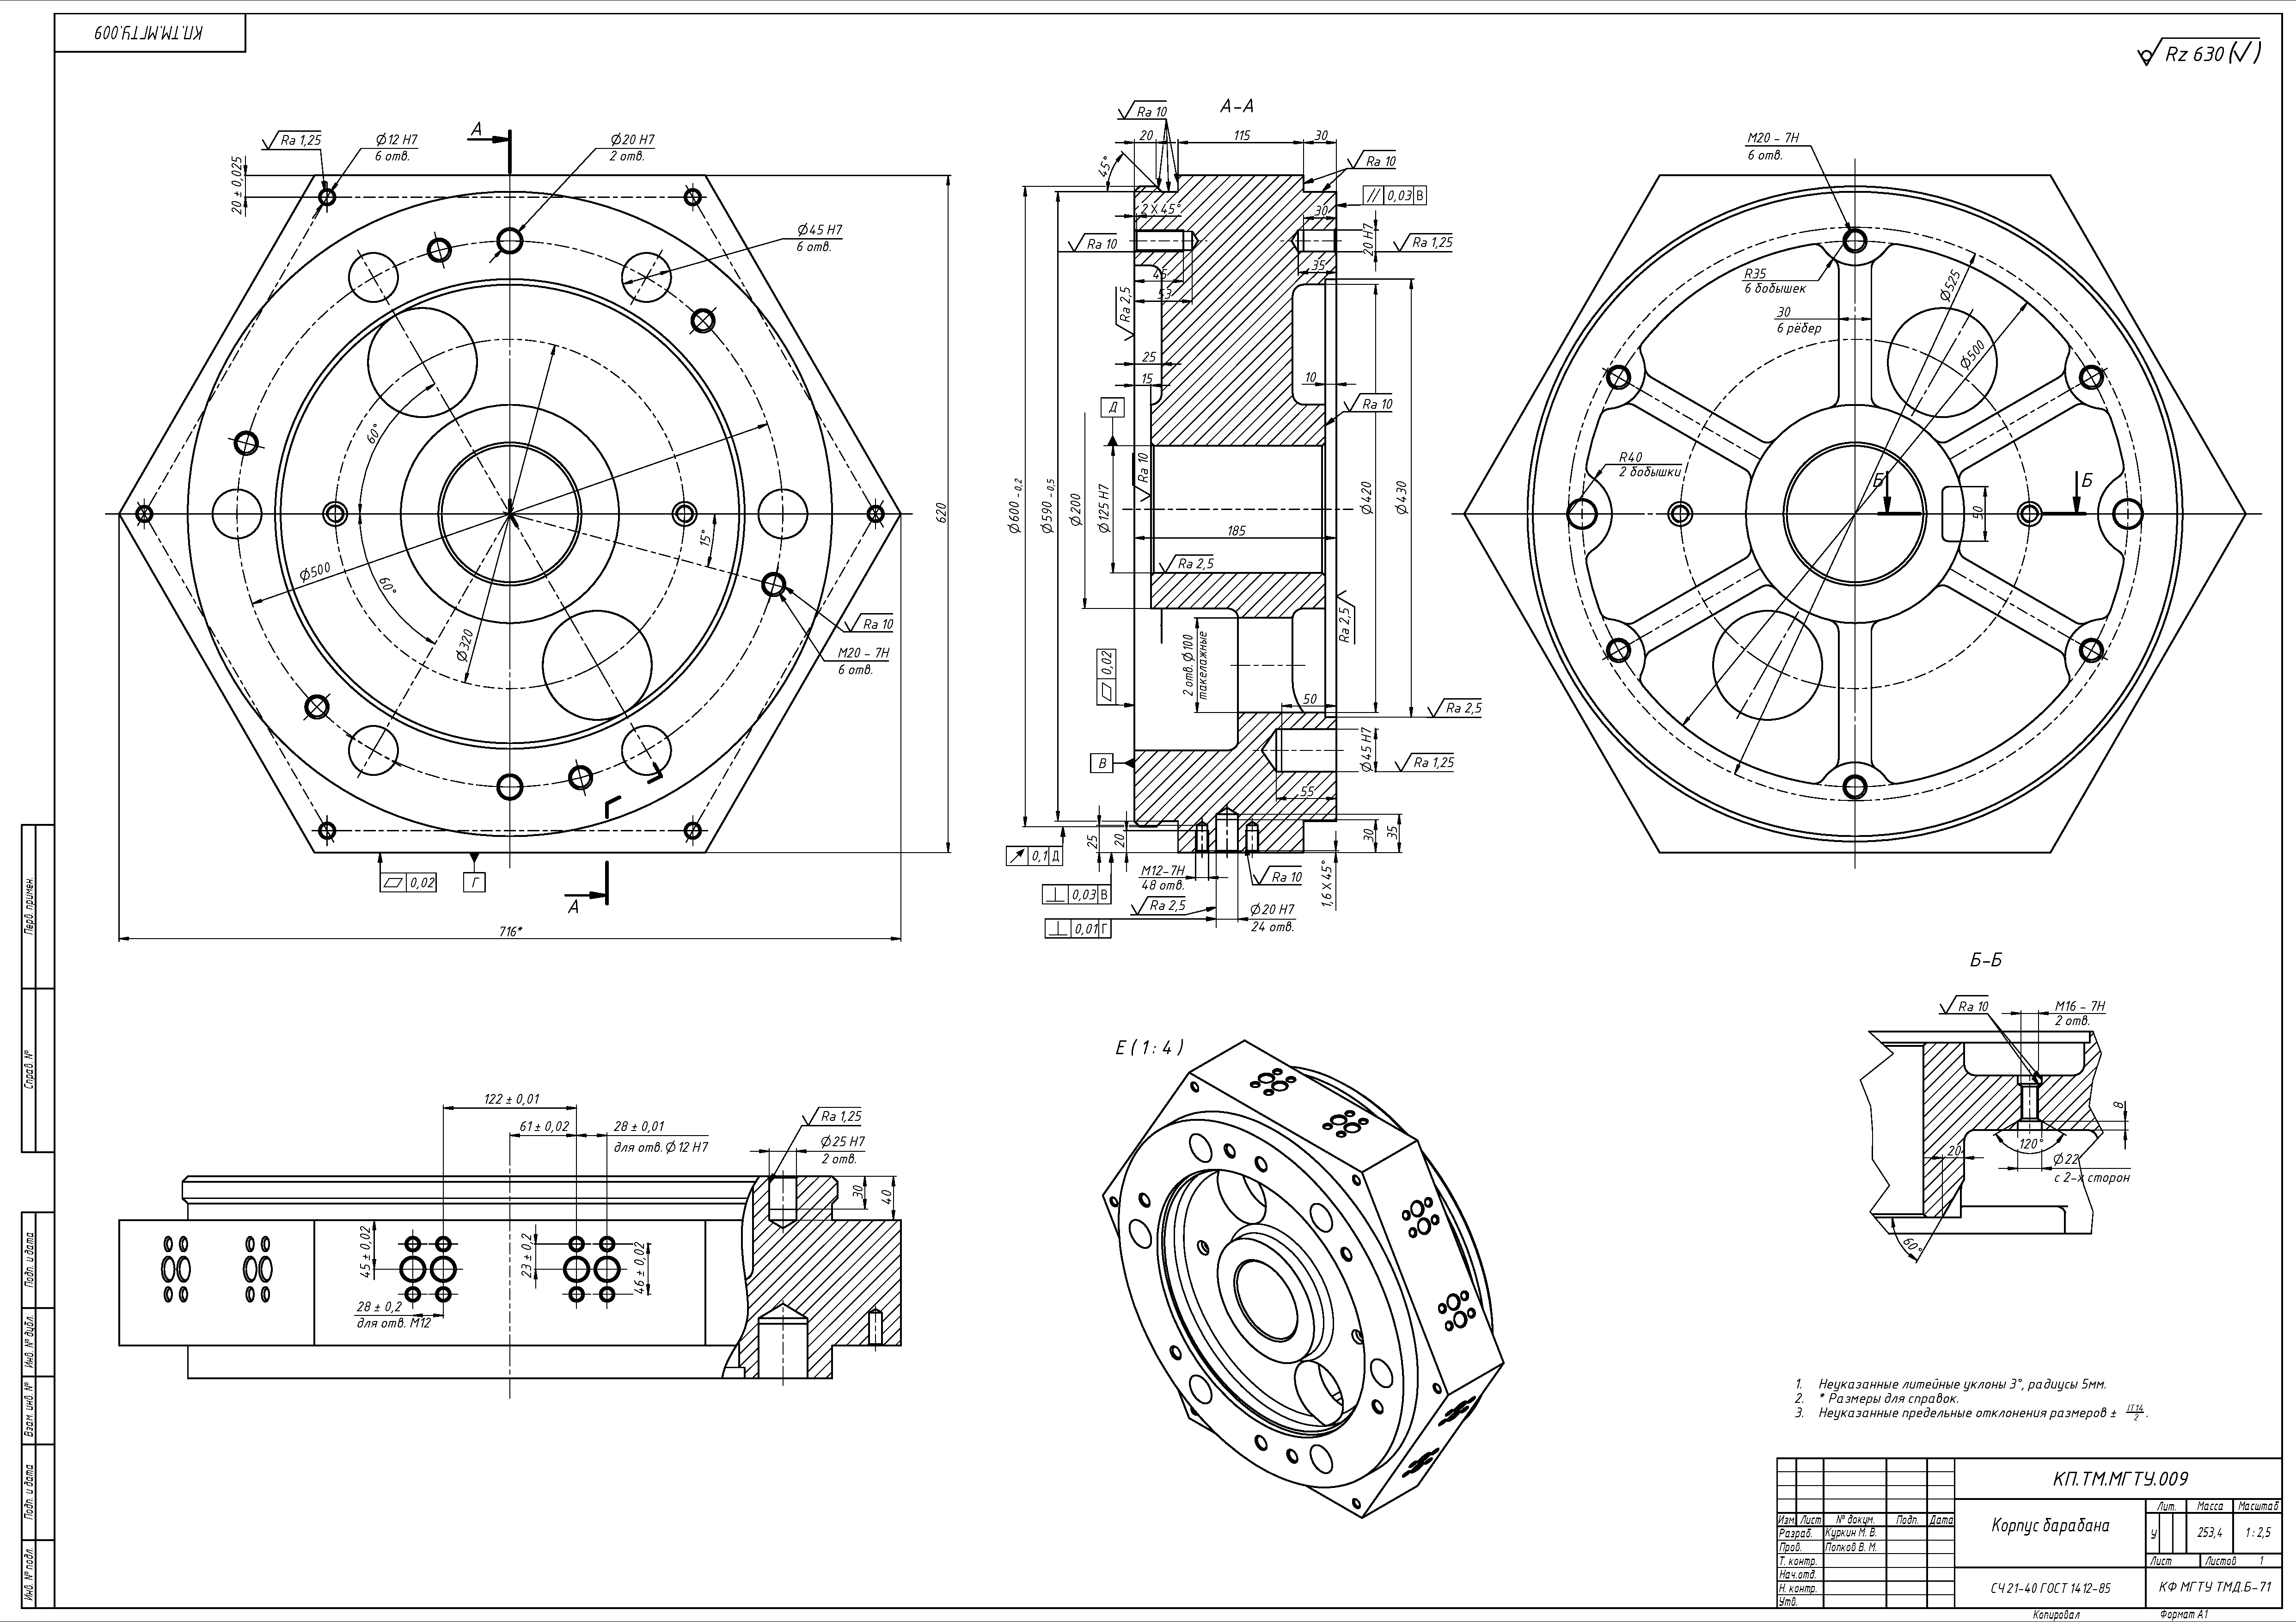
\includepdf[offset=0mm -5mm,angle=90,scale=0.8,pagecommand={\append{Чертёж детали}\label{ap:drw}}]{./graphics/drum_body.pdf}

  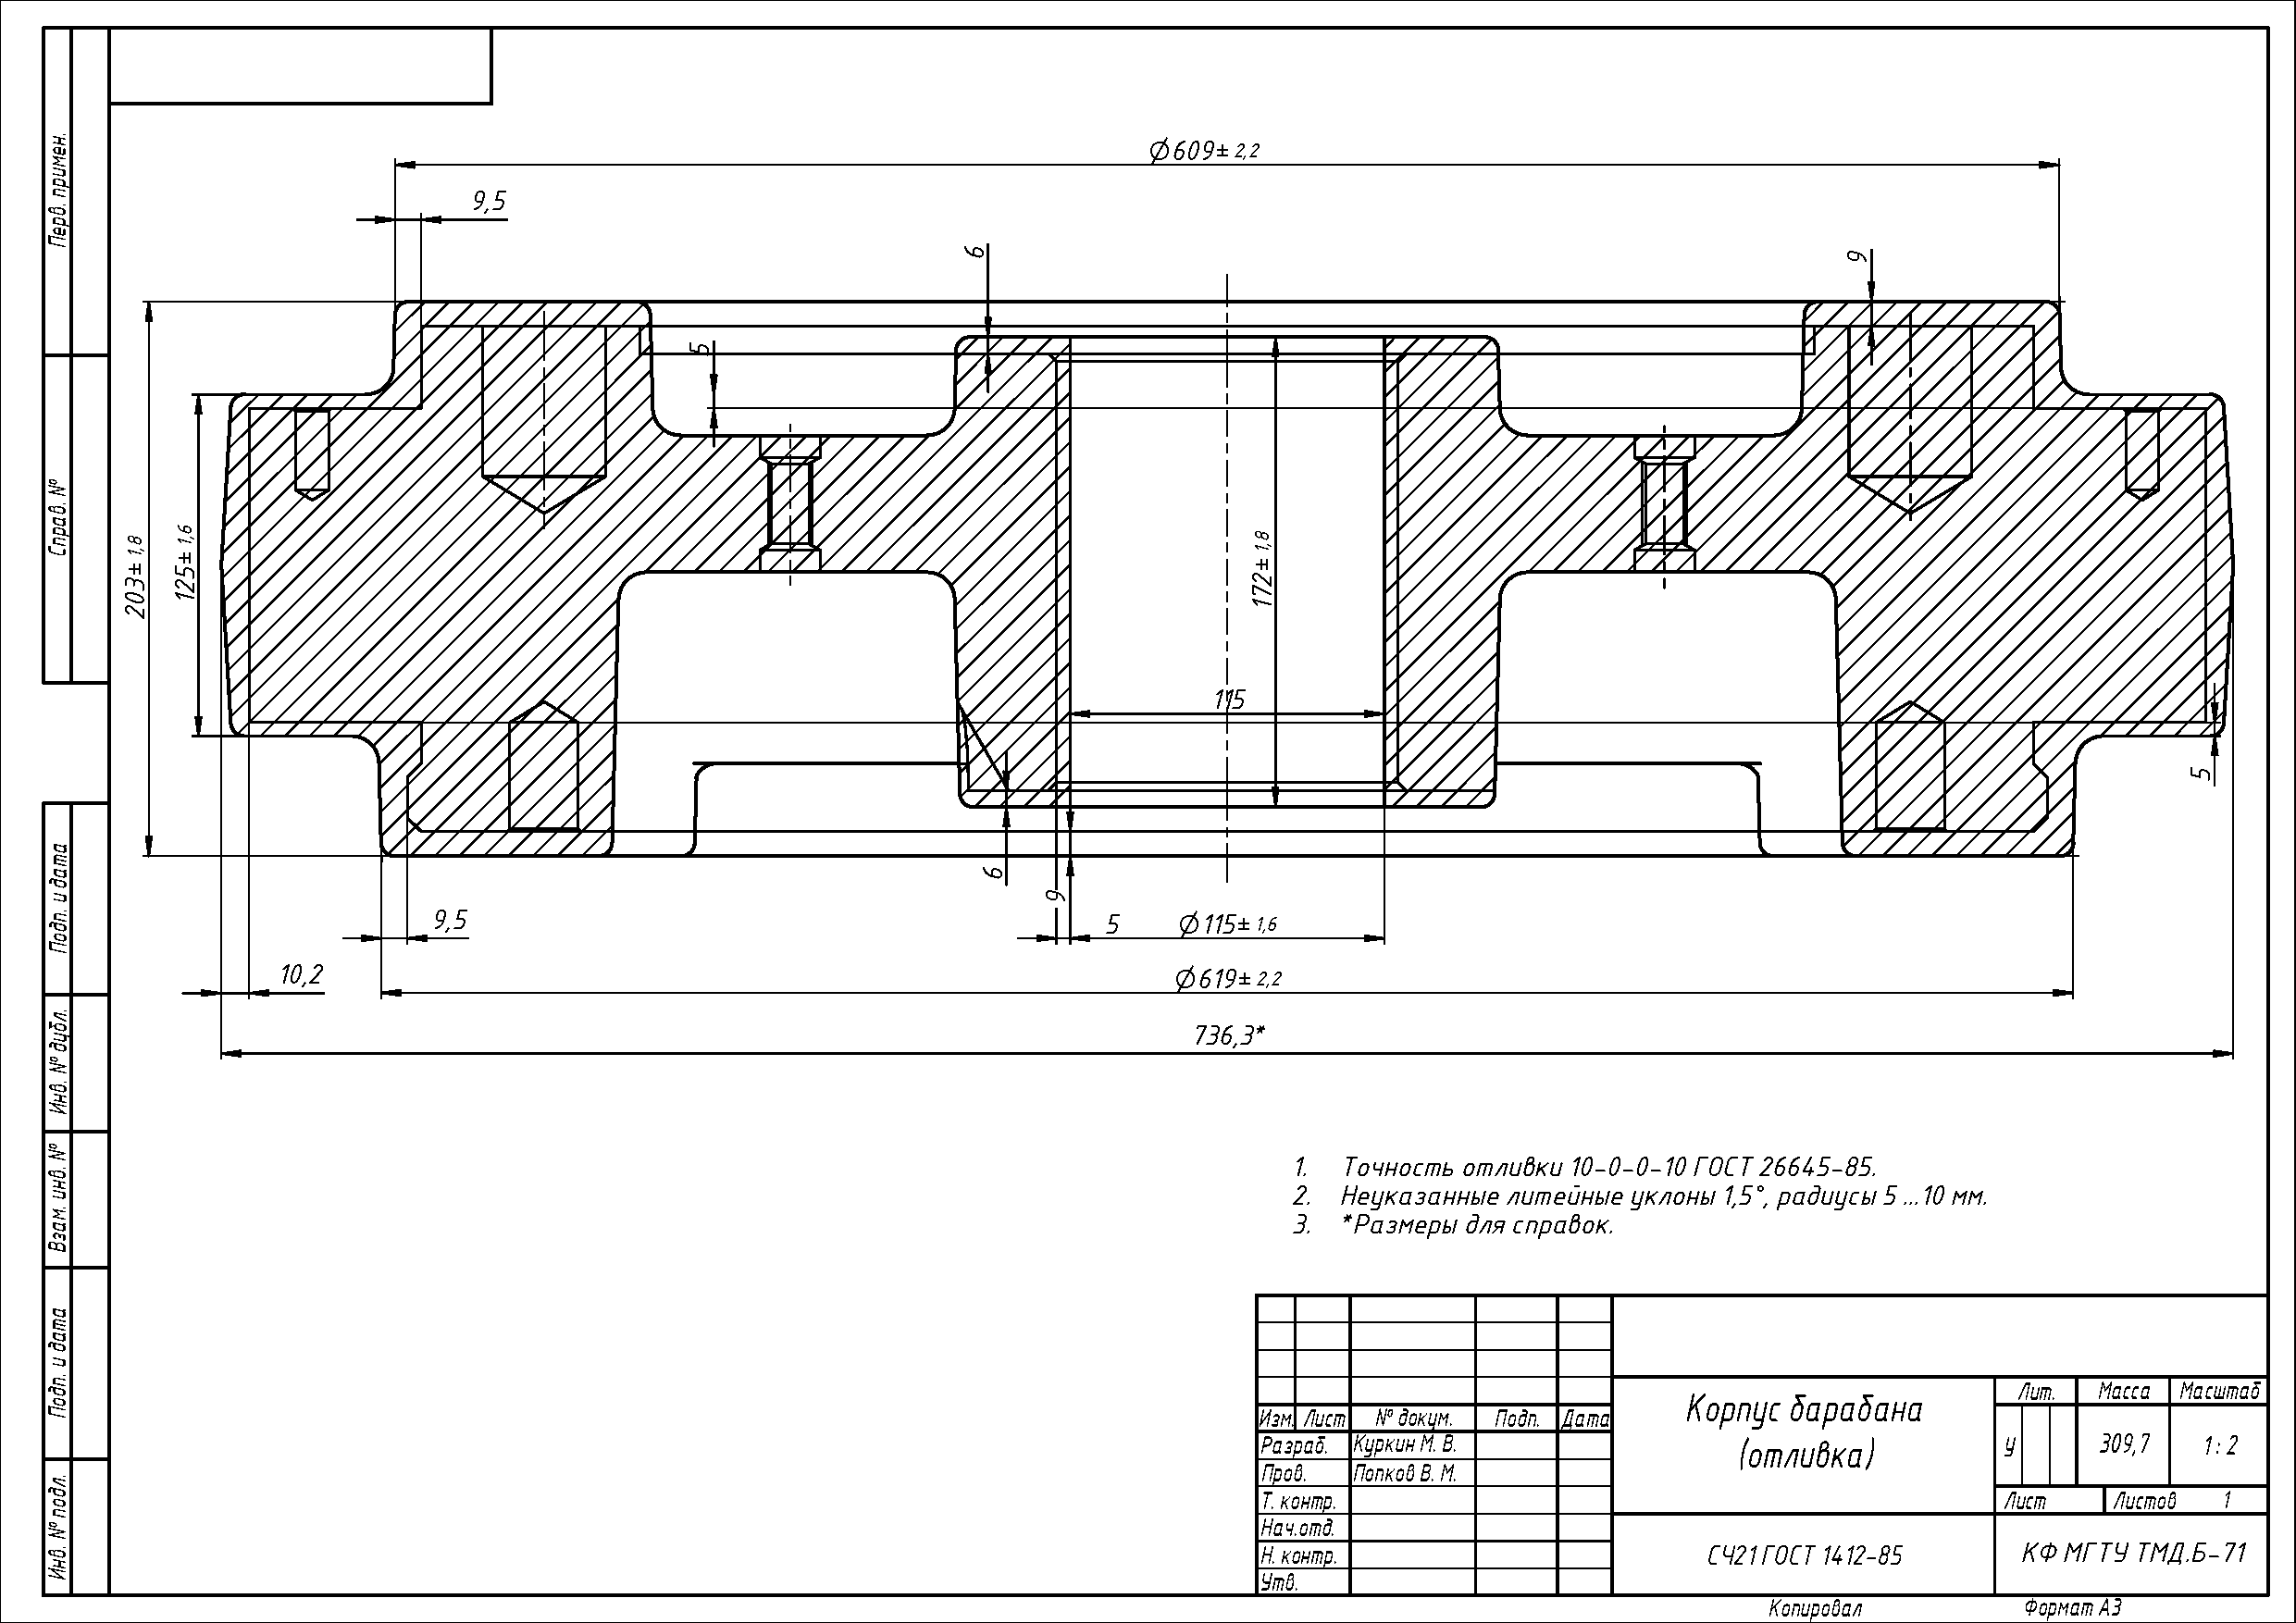
\includepdf[offset=0mm -5mm,angle=90,scale=0.8,pagecommand={\append{Чертёж заготовки}\label{ap:prt}}]{./graphics/drum_body-part.pdf}

  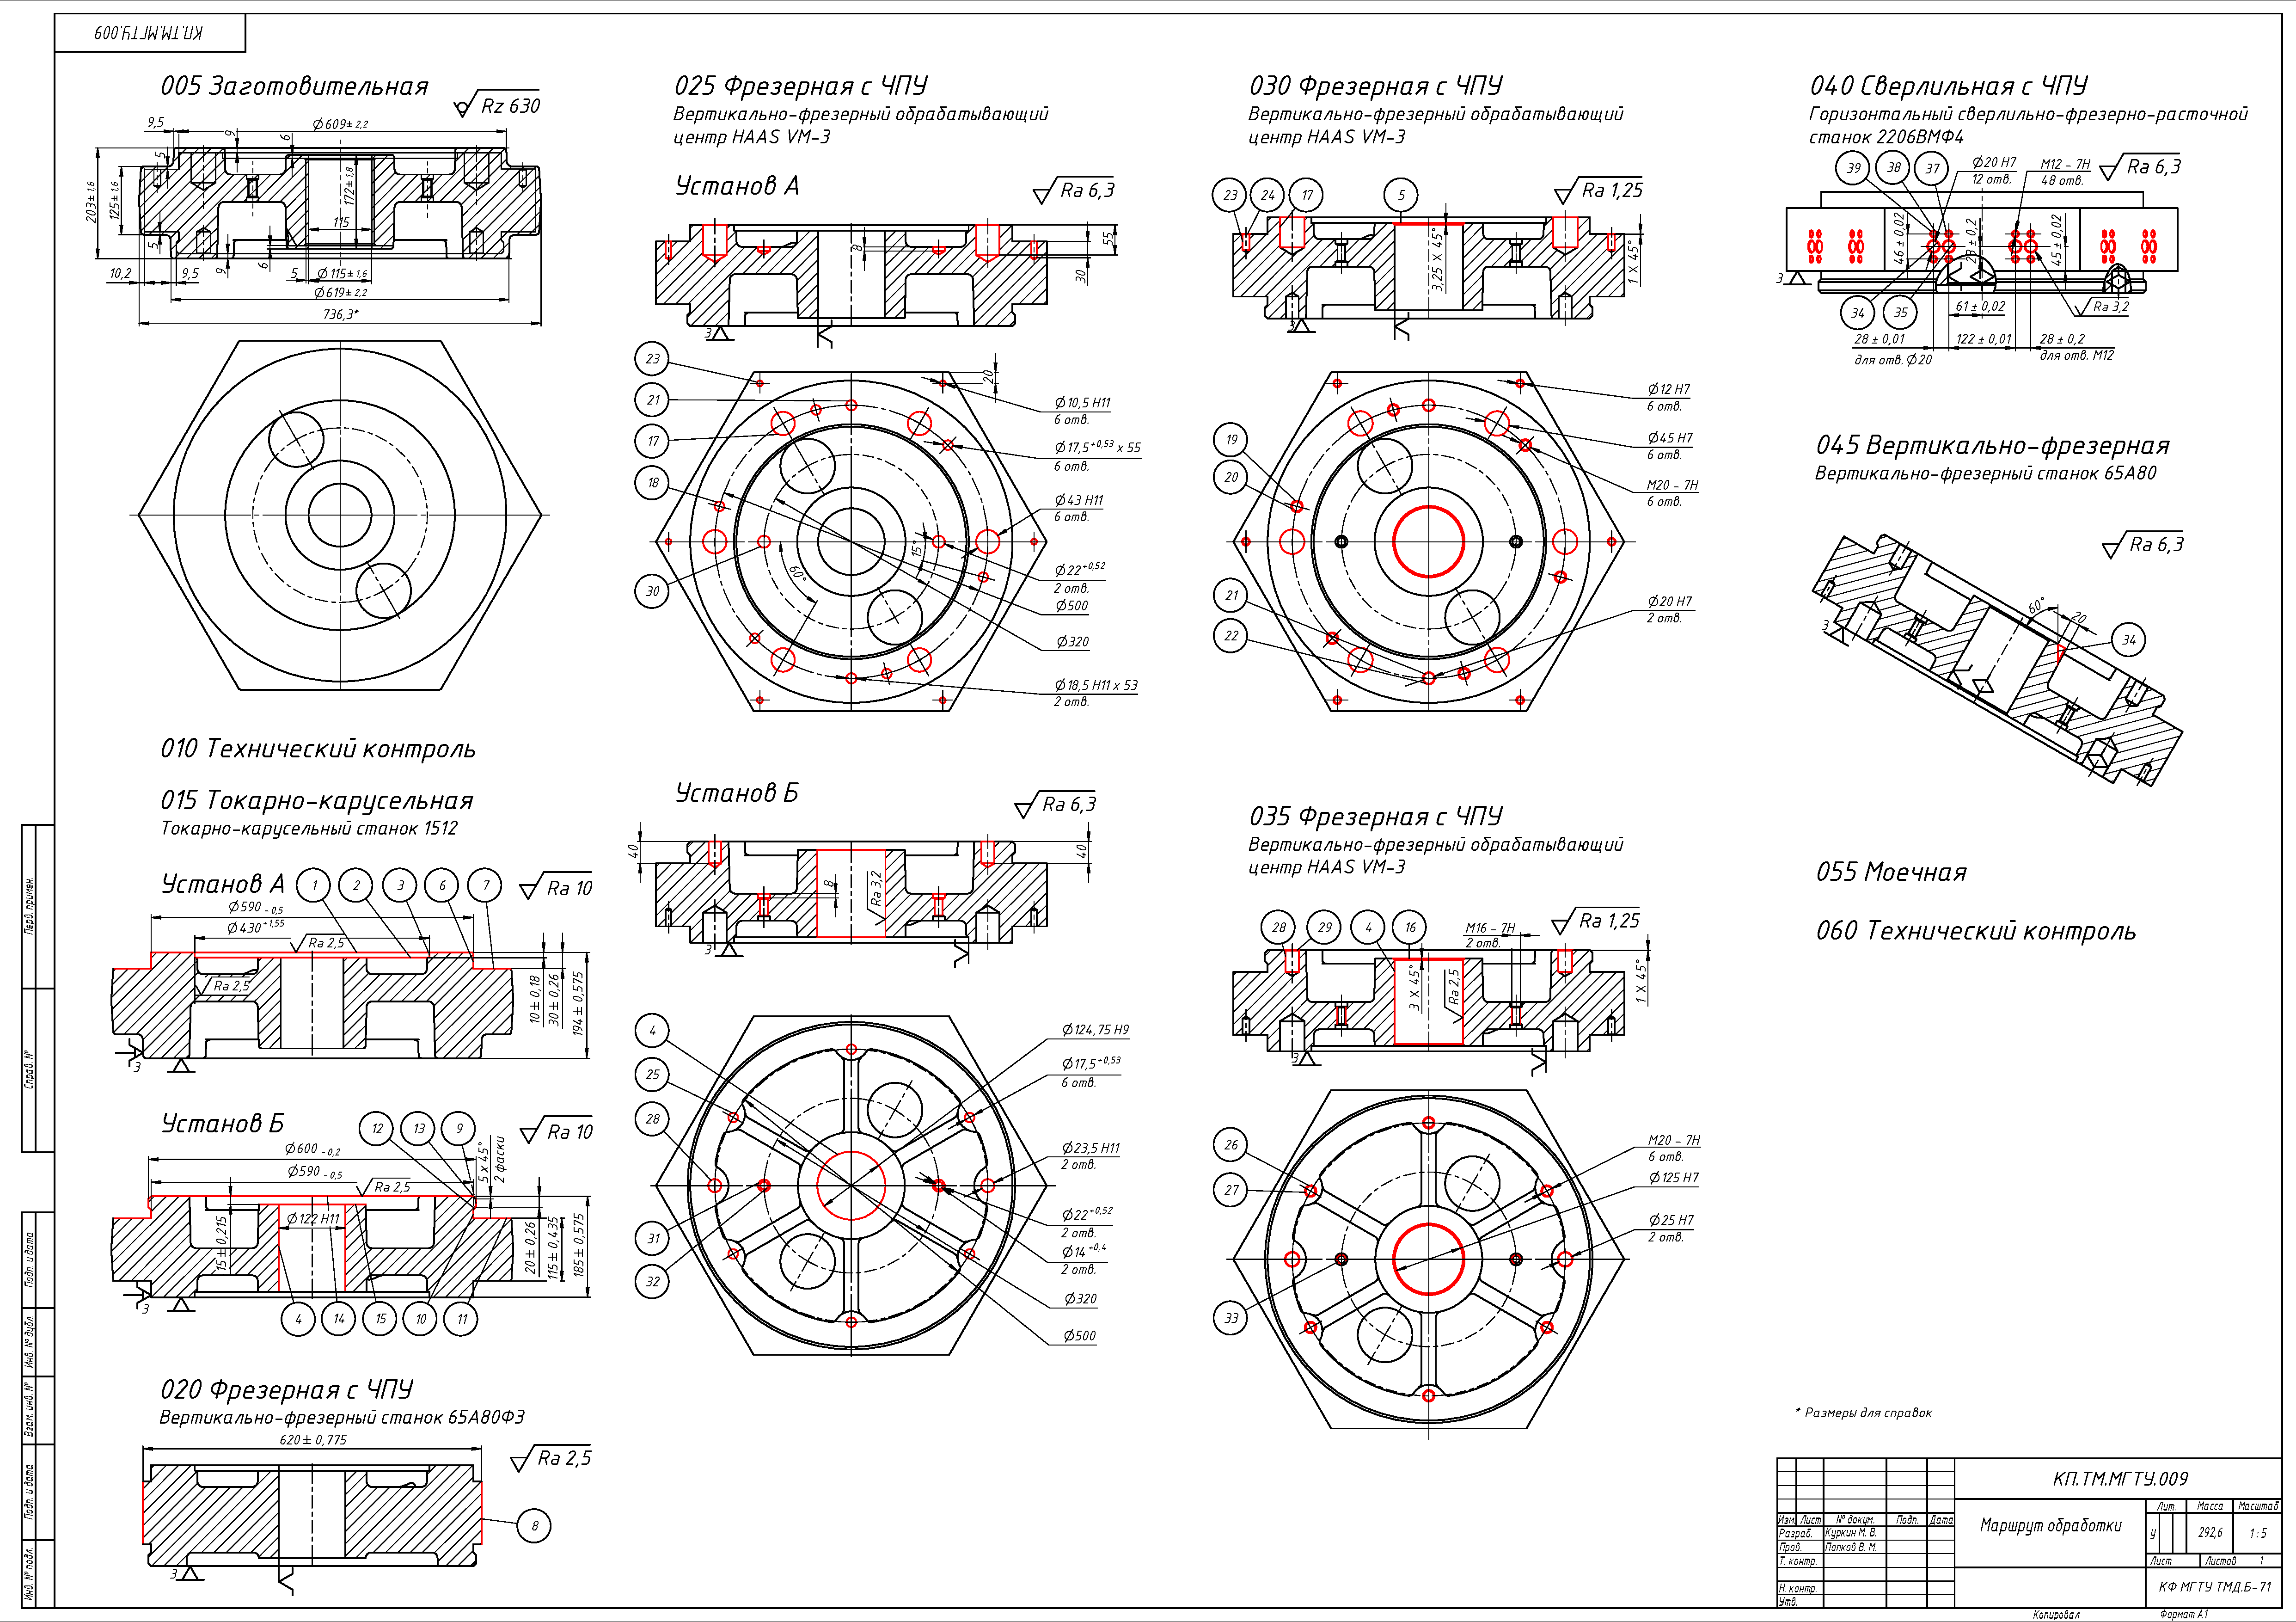
\includepdf[offset=0mm -5mm,angle=90,scale=0.8,pagecommand={\append{Маршрут обработки}\label{ap:route}}]{./graphics/machining_route.pdf}

  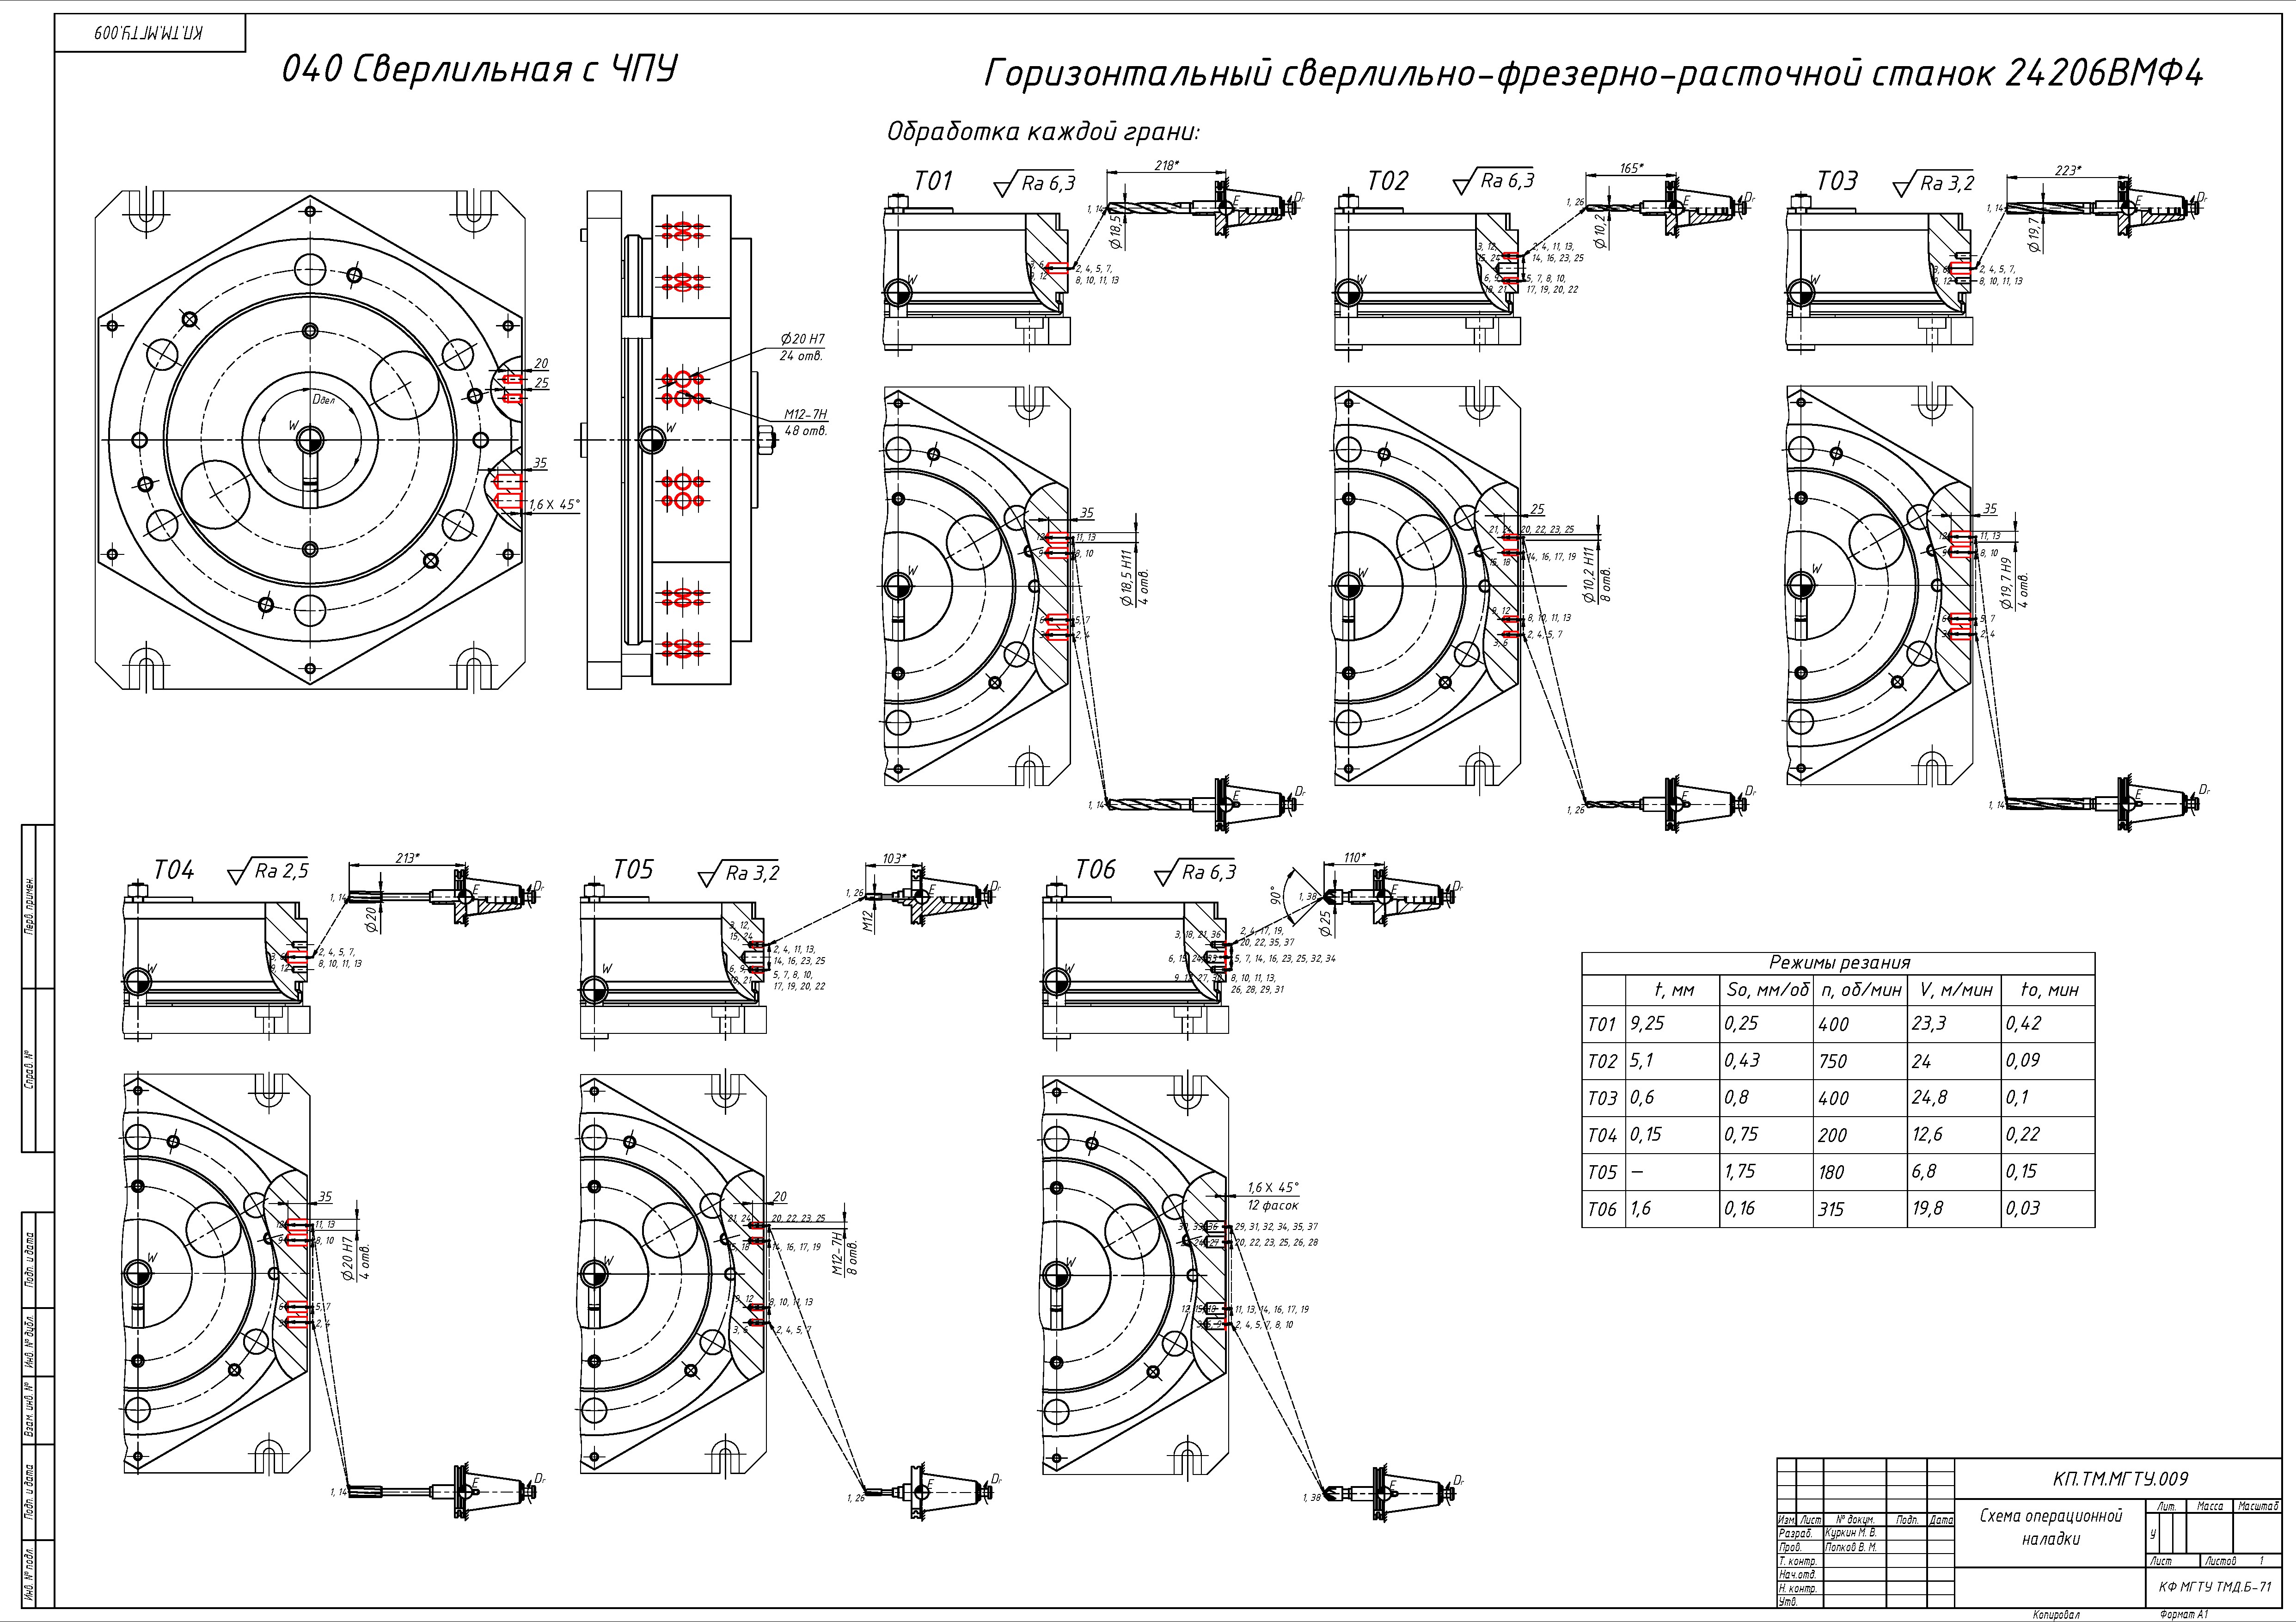
\includepdf[offset=0mm -5mm,angle=90,scale=0.8,pagecommand={\append{Схемы операционных наладок}\label{ap:nal}}]{./graphics/naladka_040.pdf}

  \includepdf[angle=90,scale=0.8,pagecommand={\fancyfoot[r]{\thepage}}]{./graphics/naladka_045.pdf}

  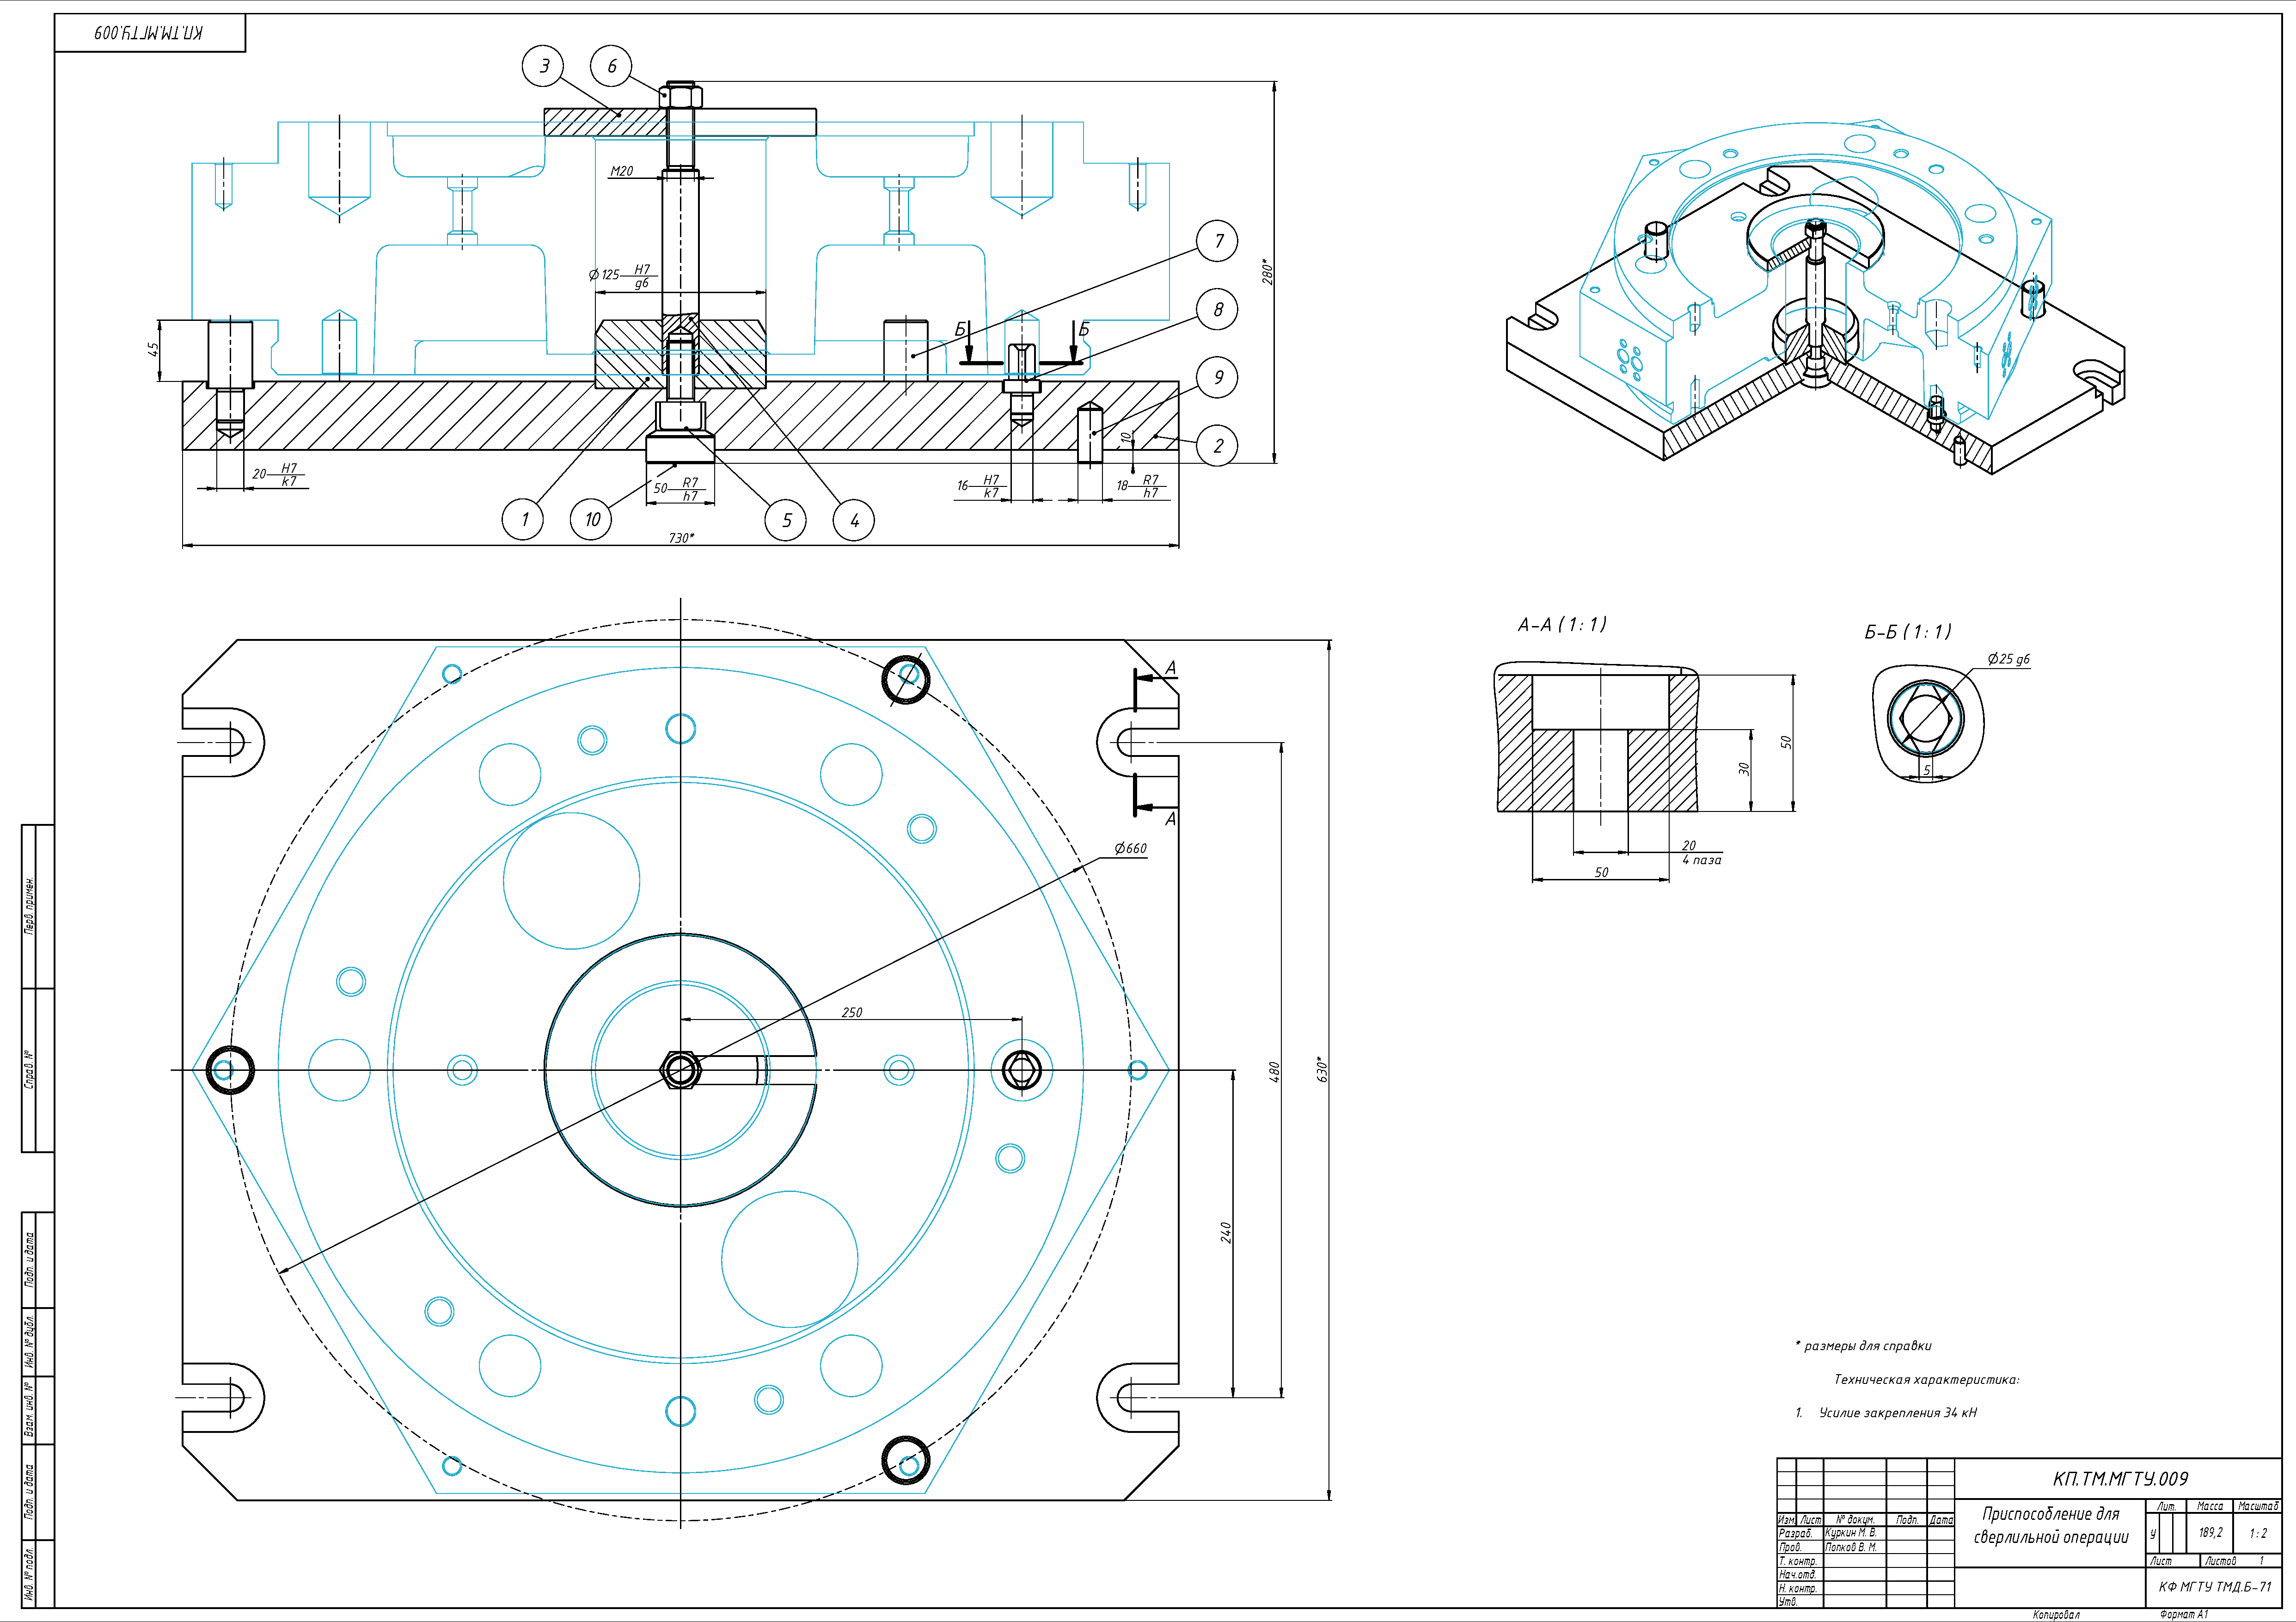
\includepdf[offset=0mm -10mm,angle=90,scale=0.8,pagecommand={\append{Сборочные чертежи приспособлений}\label{ap:rig}}]{./graphics/rig_040.pdf}

  \includepdf[angle=90,scale=0.8,pagecommand={\fancyfoot[r]{\thepage}}]{./graphics/rig_045.pdf}

  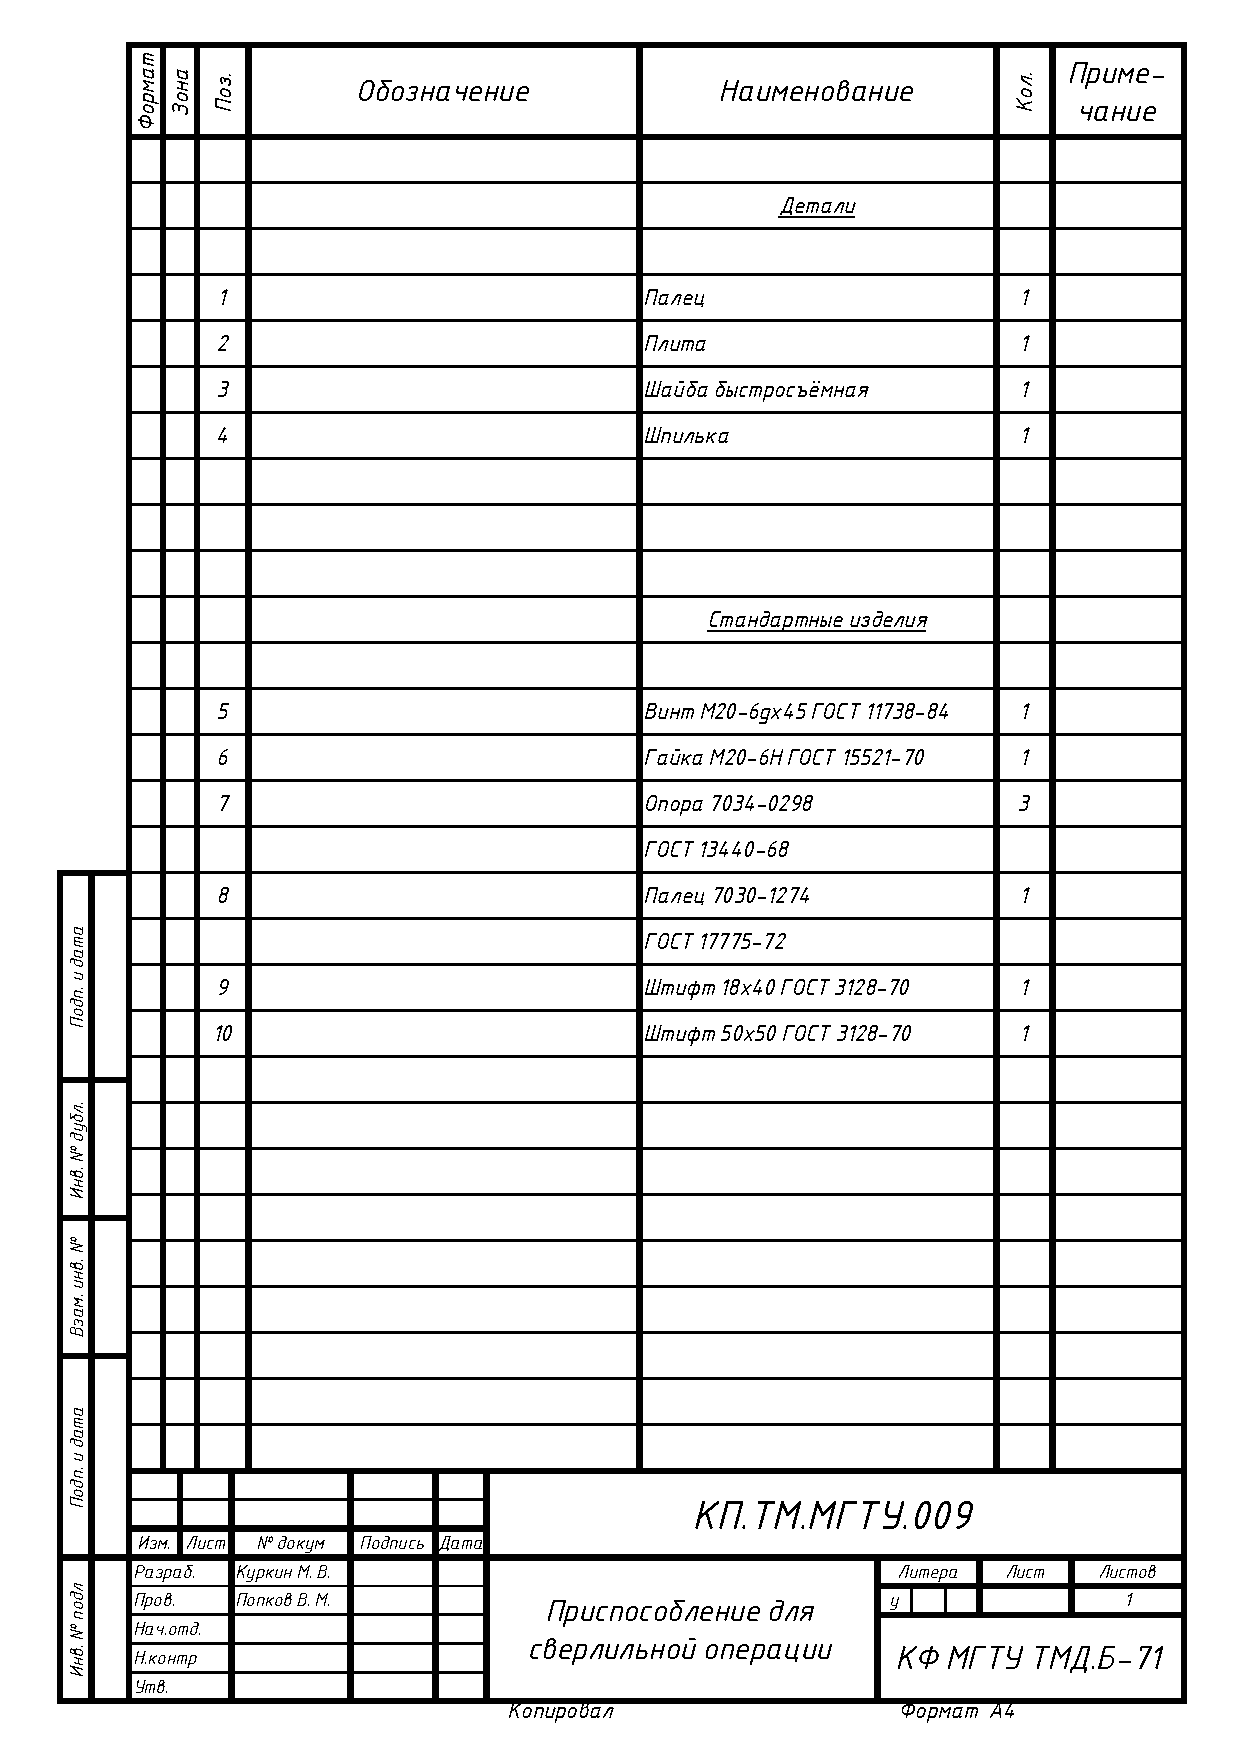
\includepdf[offset=0mm -5mm,angle=0,scale=0.8,pagecommand={\append{Спецификации}\label{ap:sp}}]{./graphics/sp_040.pdf}

  \includepdf[angle=0,scale=0.8,pagecommand={\fancyfoot[r]{\thepage}}]{./graphics/sp_045.pdf}

  \end{appendices}

\end{document}